\documentclass[11pt]{article}
\usepackage[letterpaper,margin=0.85in,headheight=14pt]{geometry}
\usepackage[T1]{fontenc}
\usepackage{lmodern}
\usepackage{microtype}
\usepackage{amsmath,amssymb,amsthm,mathtools}
\usepackage{booktabs,longtable,array,multirow}
\usepackage{enumitem}
\usepackage[dvipsnames,svgnames]{xcolor}
\usepackage{tikz}
\usetikzlibrary{arrows.meta,positioning,calc,decorations.pathreplacing}
\usepackage{fancyhdr}
\usepackage{hyperref}
\usepackage{cleveref}

\definecolor{navy}{HTML}{15324B}
\definecolor{teal}{HTML}{007C83}
\definecolor{gold}{HTML}{B57A00}
\definecolor{pale}{HTML}{F2F7F8}
\definecolor{rose}{HTML}{9A3B47}
\hypersetup{colorlinks=true,linkcolor=navy,citecolor=teal,urlcolor=teal,
  pdftitle={A Complete Mathematical Tutorial on Human-AI Productivity Paradoxes},
  pdfauthor={Prepared as teaching notes}}

\pagestyle{fancy}
\fancyhf{}
\lhead{Human--AI Productivity Paradoxes}
\rhead{Mathematical Tutorial}
\cfoot{\thepage}
\setlength{\parindent}{0pt}
\setlength{\parskip}{5pt}
\setlist{itemsep=2pt,topsep=4pt}
\allowdisplaybreaks

\newtheoremstyle{tutorial}{7pt}{7pt}{\itshape}{}{}{.}{.6em}{}
\theoremstyle{tutorial}
\newtheorem{theorem}{Theorem}[section]
\newtheorem{proposition}[theorem]{Proposition}
\newtheorem{lemma}[theorem]{Lemma}
\newtheorem{corollary}[theorem]{Corollary}
\newtheorem{definition}[theorem]{Definition}
\newtheorem{condition}[theorem]{Condition}
\theoremstyle{remark}
\newtheorem{remark}[theorem]{Remark}
\newtheorem{example}[theorem]{Example}
\newenvironment{intuition}{\begin{quote}\color{teal}\textbf{Intuition.}\ }{\end{quote}}
\newenvironment{checkpoint}{\begin{quote}\color{rose}\textbf{Checkpoint.}\ }{\end{quote}}
\newenvironment{teachingnote}{\begin{quote}\color{gold!70!black}\textbf{Teaching note.}\ }{\end{quote}}
\newcommand{\E}{\mathbb{E}}
\newcommand{\Pp}{\mathbb{P}}
\newcommand{\R}{\mathbb{R}}
\newcommand{\1}{\mathbb{I}}
\newcommand{\pos}[1]{\left(#1\right)_{+}}
\newcommand{\calP}{\mathcal{P}}
\newcommand{\calE}{\mathcal{E}}
\newcommand{\dd}{\,\mathrm{d}}
\newcommand{\sgn}{\operatorname{sgn}}

\title{\vspace{-1.2cm}\textbf{A Complete Mathematical Tutorial on\\Human--AI Productivity Paradoxes}\\[5pt]
\large Skill, Effort, Unreliability, and AI Literacy}
\author{Teaching notes for Aouad, Lykouris, and Zhong (2026)}
\date{Version prepared from arXiv:2605.11350v1\\[2pt]
\small Scope: main paper and mathematical supplements A--C; the convex-cost extension is omitted}

\begin{document}
\maketitle

\begin{abstract}
These notes rebuild the paper's mathematical argument from first principles.  Every optimization step,
stationary-distribution calculation, derivative decomposition, threshold comparison, and mode argument
needed for the three main results is written out.  The central message is that AI is locally productive
at a fixed skill, yet can lower aggregate or expected productivity through endogenous effort: effort affects
future skill, responds to unreliable assistance, and interacts with skill-dependent verification ability.
The notes are designed to support a graduate lecture sequence and include diagnostic checks, worked special
cases, proof roadmaps, and exercises with solutions.  Appendix D of the paper, which extends the model to
convex effort costs, is intentionally outside the scope requested for these notes.
\end{abstract}

\tableofcontents
\newpage

\section{How to read the paper}

\subsection{The three feedback loops}

All of the paper's results begin with the same static choice: an agent with skill $s$ chooses costly effort
$e$ in the presence of AI assistance.  The three main sections add one feedback loop at a time.

\begin{center}
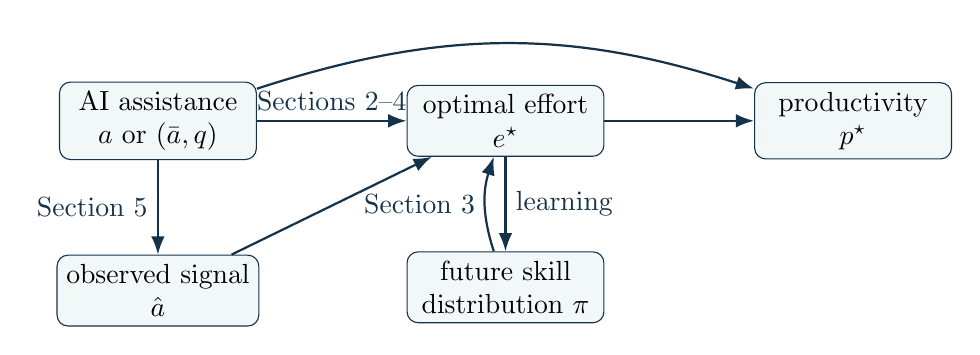
\begin{tikzpicture}[>=Latex,node distance=12mm and 19mm,
  box/.style={draw=navy,rounded corners,fill=pale,minimum width=25mm,minimum height=9mm,align=center},
  arr/.style={->,thick,navy}]
\node[box] (ai) {AI assistance\\$a$ or $(\bar a,q)$};
\node[box,right=of ai] (eff) {optimal effort\\$e^\star$};
\node[box,right=of eff] (prod) {productivity\\$p^\star$};
\node[box,below=of eff] (skill) {future skill\\distribution $\pi$};
\node[box,below=of ai] (signal) {observed signal\\$\hat a$};
\draw[arr] (ai)--node[above]{Sections 2--4}(eff);
\draw[arr] (eff)--(prod);
\draw[arr] (ai) to[bend left=18] (prod);
\draw[arr] (eff)--node[right]{learning}(skill);
\draw[arr] (skill) to[bend left=18] node[left]{Section 3} (eff);
\draw[arr] (ai)--node[left]{Section 5}(signal);
\draw[arr] (signal)--(eff);
\end{tikzpicture}
\end{center}

The logical order is therefore:
\begin{enumerate}
  \item solve the deterministic static optimization exactly;
  \item let effort control upward movement in a birth--death skill process;
  \item make AI assistance random and differentiate through the endogenous optimizer;
  \item let skill determine signal accuracy, then feed expected effort back into skill dynamics.
\end{enumerate}

\subsection{Main results and proof dependencies}

\begin{longtable}{p{0.17\textwidth}p{0.31\textwidth}p{0.42\textwidth}}
\toprule
Result & Economic statement & Mathematical engine\\
\midrule
\endhead
Basic model & AI replaces effort and weakly raises productivity at fixed skill. & Concavity of
$p(x)-\gamma x$ and a change of variable from effort to total input.\\
Theorem 1 & With endogenous learning, productivity may rise and then fall within a fixed activity regime. &
Detailed balance; first-order stochastic dominance; a quotient derivative; a single-crossing result;
large-$\mu$ asymptotics governed by the sensitivity gap $\Delta_m$.\\
Theorem 2 & With unreliable AI, IARA gives a decreasing-then-increasing profile, while DARA gives an increasing profile. &
Implicit differentiation of the effort FOC and factorization by the Arrow--Pratt coefficient
$A(x)=-p''(x)/p'(x)$.\\
Theorem 3 & Skill-dependent AI literacy can produce multiple modes in the long-run skill distribution. &
Bayes' rule; piecewise effort formulas; non-monotonicity in skill; the identity
$\pi_{k+1}/\pi_k=\lambda(e_k)/\mu$.\\
\bottomrule
\end{longtable}

\subsection{Assumptions that do real work}

The main analysis assumes:
\begin{enumerate}
  \item $s,e,a\ge 0$ enter production additively as $x=s+e+a$;
  \item $p$ is nonnegative, increasing, continuous, twice differentiable where required, and concave;
  \item effort cost is linear, $c(e)=\gamma e$, $\gamma>0$;
  \item agents are myopic: current effort does not internalize future skill;
  \item in the dynamic model, $\lambda(e)>0$ is increasing (and, in Section 3, concave and differentiable);
  \item skill decays at the constant rate $\mu>0$.
\end{enumerate}
The linear cost is important for the exact flat region of state-level productivity.  The paper's convex-cost
extension is not treated here.

\section{Mathematical toolkit}

\subsection{Concavity and the largest maximizer}

Let $g(x)=p(x)-\gamma x$.  Since $p$ is concave, $g$ is concave.  The paper assumes
\[
  \limsup_{x\to\infty}\frac{p(x)}{x}<\gamma,
\]
so $g(x)\to-\infty$ at least along the tail strongly enough to make the argmax nonempty and bounded.
Define the largest maximizer
\[
  x^\star:=\max\arg\max_{x\ge0}\{p(x)-\gamma x\}.
\]
For differentiable $p$, concavity gives the useful slope characterization
\[
  p'(x^\star)\ge\gamma,
  \qquad p'(x^\star+\varepsilon)<\gamma\quad(\varepsilon>0).
\]
If $p'(x)=\gamma$ over an interval, selecting the largest maximizer chooses its right endpoint.  This
tie-breaking rule is why all later formulas use $x^\star$ unambiguously.

\subsection{Finite birth--death chains}

For states $1,\ldots,N$, let the upward rate from $k$ to $k+1$ be $b_k>0$ and the downward rate from
$k+1$ to $k$ be $d_{k+1}>0$.  At stationarity, detailed balance is
\[
  \pi_k b_k=\pi_{k+1}d_{k+1}.
\]
Hence, recursively,
\[
  \frac{\pi_{k+1}}{\pi_k}=\frac{b_k}{d_{k+1}},\qquad
  \pi_k=\pi_1\prod_{i=1}^{k-1}\frac{b_i}{d_{i+1}}.
\]
Normalization $\sum_k\pi_k=1$ yields
\[
  \pi_1=\left(1+\sum_{k=2}^{N}\prod_{i=1}^{k-1}\frac{b_i}{d_{i+1}}\right)^{-1}.
\]
This identity is used twice: first with $b_k=\lambda(e^\star(s_k,a))$, then with
$b_k=\lambda(e_b^\star(s_k,\bar a,q))$.

\subsection{First-order stochastic dominance on ordered states}

For ordered skills $s_1\le\cdots\le s_N$, distribution $X$ first-order stochastically dominates $Y$ if
\[
  \sum_{i=1}^k \Pp(X=s_i)\le \sum_{i=1}^k\Pp(Y=s_i),\qquad k=1,\ldots,N.
\]
The inequality points this way because the left side is the probability of being in one of the \emph{lowest}
$k$ states.  Smaller lower-tail probabilities mean more mass on high skill.

\subsection{ARA and a derivative identity}

For $p'>0$, define
\[
  A(x):=-\frac{p''(x)}{p'(x)}.
\]
Concavity implies $A(x)\ge0$.  IARA means $A$ increases; DARA means it decreases.  Equivalently,
$A(x)=-(\log p'(x))'$, so ARA is the instantaneous proportional rate at which marginal productivity falls.

\subsection{Modes from adjacent probability ratios}

For any strictly positive discrete distribution,
\[
  r_k:=\frac{\pi_{k+1}}{\pi_k}
\]
determines local direction: $r_k>1$ means the mass rises from $k$ to $k+1$, while $r_k<1$ means it falls.
A decreasing sequence $r_k$ crosses $1$ at most once, hence gives a unimodal distribution.  Multiple
crossings of $1$ allow multiple peaks.  This observation is the bridge from effort non-monotonicity to skill
polarization.

\section{The deterministic basic model}

\subsection{Primitives and the agent's problem}

The agent has skill $s\ge0$, chooses effort $e\ge0$, and receives deterministic AI assistance $a\ge0$.
Total input and utility are
\[
  x=s+e+a,
  \qquad u(e;s,a)=p(s+e+a)-\gamma e.
\]
Productivity excludes effort cost:
\[
  p^\star(s,a)=p(s+e^\star(s,a)+a).
\]
This distinction matters: utility is the choice criterion; productivity is the outcome the paper evaluates.

\subsection{Full solution of the optimization problem}

\paragraph{Step 1: rewrite the decision in terms of total input.}
Set $x=s+e+a$.  Before the agent exerts any effort, skill and AI already provide the baseline input
$s+a$.  Effort can only add to this baseline because $e\ge0$.  Therefore the feasible total inputs satisfy
\[
  x=s+a+e\ge s+a.
\]
Equivalently, $e=x-s-a$ and $e\ge0$ if and only if $x\ge s+a$.  The optimization problem becomes
\begin{align*}
  \max_{e\ge0}\{p(s+e+a)-\gamma e\}
  &=\max_{x\ge s+a}\{p(x)-\gamma(x-s-a)\}\\
  &=\gamma(s+a)+\max_{x\ge s+a}\{p(x)-\gamma x\}.
\end{align*}
The first term, $\gamma(s+a)$, does not depend on $x$, so it does not affect which $x$ is optimal.  Thus
we maximize the concave function
\[
  g(x)=p(x)-\gamma x
\]
over the feasible interval $[s+a,\infty)$.  Recall that $x^\star$ is the largest maximizer of $g$ over all
$x\ge0$.  In words, $x^\star$ is the total input the agent would like to reach if the baseline $s+a$ did
not restrict the choice.

\paragraph{Step 2: determine the optimal total input.}
There are two cases.

\paragraph{Case 1: $s+a\le x^\star$.}
The desired total input $x^\star$ is feasible because it is at least as large as the baseline $s+a$.
The agent supplies exactly the missing amount through effort:
\[
  x^{\mathrm{opt}}=x^\star,
  \qquad
  e^\star=x^{\mathrm{opt}}-(s+a)=x^\star-s-a\ge0.
\]

\paragraph{Case 2: $s+a>x^\star$.}
The baseline input has already passed the desired level $x^\star$.  Reaching $x^\star$ would require
\[
  e=x^\star-s-a<0,
\]
which is impossible because effort must satisfy $e\ge0$.  Moreover, every positive effort would push total
input even farther to the right of $x^\star$.  Concavity makes $g(x)=p(x)-\gamma x$ weakly decreasing to
the right of its largest maximizer, so moving farther right cannot improve utility.  The best feasible choice
is therefore the smallest feasible total input, obtained by choosing no effort:
\[
  x^{\mathrm{opt}}=s+a,
  \qquad
  e^\star=0.
\]

The two cases can be summarized by one expression:
\begin{equation}
  \boxed{x^{\mathrm{opt}}=\max\{x^\star,s+a\}.}
  \label{eq:optimal-total-input}
\end{equation}
The maximum appears because the agent would like total input $x^\star$, but total input can never be below
the amount $s+a$ that skill and AI already provide.

\paragraph{Step 3: what does the subscript ``$+$'' mean?}
For any real number $z$, its \emph{positive part} is defined as
\[
  z_+:=\max\{z,0\}
  =\begin{cases}
      z,&\text{if }z\ge0,\\
      0,&\text{if }z<0.
    \end{cases}
\]
The small $+$ is a subscript attached to the entire expression.  It does \emph{not} mean that we add an
extra number.  It means: ``keep the expression if it is nonnegative; otherwise replace it by zero.''  For
example,
\[
  (3)_+=3,
  \qquad
  (0)_+=0,
  \qquad
  (-4)_+=0.
\]

\paragraph{Step 4: derive the optimal-effort formula.}
Effort is the difference between optimal total input and the baseline input:
\begin{align*}
e^\star(s,a)
&=x^{\mathrm{opt}}-(s+a)\\
&=\max\{x^\star,s+a\}-(s+a)\\
&=\max\{x^\star-s-a,0\}\\
&=(x^\star-s-a)_+.
\end{align*}
The third line uses the elementary identity
\[
  \max\{A,B\}-B=\max\{A-B,0\}.
\]
Thus the positive-part symbol enforces the feasibility condition $e\ge0$ automatically:
\[
e^\star(s,a)=
\begin{cases}
x^\star-s-a,&\text{if }s+a\le x^\star,\\
0,&\text{if }s+a>x^\star.
\end{cases}
\]

\paragraph{Step 5: derive the optimal-productivity formula.}
Productivity is production evaluated at the optimal total input, without subtracting effort cost.  Using
\eqref{eq:optimal-total-input},
\begin{align*}
p^\star(s,a)
&=p(s+e^\star(s,a)+a)\\
&=p(x^{\mathrm{opt}})\\
&=p\bigl(\max\{x^\star,s+a\}\bigr).
\end{align*}
Because $p$ is weakly increasing, applying $p$ to the larger of two inputs produces the larger of the two
output values:
\[
  p\bigl(\max\{x^\star,s+a\}\bigr)
  =\max\{p(x^\star),p(s+a)\}.
\]
Equivalently, the productivity formula is
\[
p^\star(s,a)=
\begin{cases}
p(x^\star),&\text{if }s+a\le x^\star,\\
p(s+a),&\text{if }s+a>x^\star.
\end{cases}
\]
In the first case, effort fills the exact gap between $s+a$ and $x^\star$, so total input equals
$x^\star$.  In the second case, effort is zero, so total input remains $s+a$.

Combining the cases gives the paper's Proposition 2.1:
\begin{proposition}[Deterministic optimizer]
\[
  \boxed{e^\star(s,a)=\pos{x^\star-s-a}},
  \qquad
  \boxed{p^\star(s,a)=\max\{p(x^\star),p(s+a)\}}.
\]
\end{proposition}

\begin{checkpoint}
The symbol $(x^\star-s-a)_+$ says that effort equals the missing input whenever a positive gap remains, and
equals zero once skill plus AI already meet or exceed the target.  When $s+a<x^\star$, an additional unit
of AI reduces the gap, and hence effort, by exactly one unit; total input stays at $x^\star$, so productivity
stays at $p(x^\star)$.  When $s+a>x^\star$, effort is already zero and additional AI raises total input and
productivity directly.
\end{checkpoint}

\begin{example}[Reading the positive-part formula]
Suppose $x^\star=5$.
\begin{itemize}
  \item If $s=2$ and $a=1$, then the baseline is $s+a=3$ and the missing input is $5-3=2$.  Hence
  $e^\star=(5-2-1)_+=2$, total input is $2+2+1=5$, and productivity is $p(5)$.
  \item If $s=4$ and $a=2$, then the baseline is $s+a=6$, already above the target.  The raw expression
  $5-4-2=-1$ would prescribe negative effort, which is infeasible.  The positive part replaces it by zero:
  $e^\star=(-1)_+=0$.  Total input is $6$, and productivity is $p(6)$.
\end{itemize}
\end{example}

\subsection{A concrete example}

Take $p(x)=\alpha\log(1+x)$, $0<\gamma<\alpha$.  The FOC $p'(x)=\alpha/(1+x)=\gamma$ gives
\[
  x^\star=\frac{\alpha}{\gamma}-1.
\]
Hence
\[
e^\star(s,a)=\pos{\frac{\alpha}{\gamma}-1-s-a},
\quad
p^\star(s,a)=\alpha\log\!\left(1+\max\left\{\frac{\alpha}{\gamma}-1,s+a\right\}\right).
\]
This example makes the kink at $s+a=x^\star$ transparent.

\section{Endogenous skill development and the first paradox}

\subsection{The continuous-time skill process}

Let $S=(s_1,\ldots,s_N)$ with $s_1\le\cdots\le s_N$.  At state $s_k$, the myopic agent chooses
\[
  e_k(a):=e^\star(s_k,a)=\pos{x^\star-s_k-a}.
\]

\paragraph{What is a transition rate?}
The model runs in \emph{continuous time}: an agent can remain at the same skill level for some time and then
move randomly to another level.  A transition rate describes how quickly such moves arrive.  Economists
encounter the same object as a job-separation hazard, a default intensity, a Poisson arrival rate, or a
depreciation hazard.

Formally, suppose an agent is currently at state $s_i$ and let $r_{ij}$ be the transition rate from $s_i$ to
$s_j$.  Over a very short interval of length $h$,
\begin{equation}
\Pp\bigl(S(t+h)=s_j\mid S(t)=s_i\bigr)=r_{ij}h+o(h),
\qquad i\ne j.
\label{eq:transition-rate-definition}
\end{equation}
The notation $o(h)$ represents terms that become negligible relative to $h$: formally,
$o(h)/h\to0$ as $h\downarrow0$.  Thus, for a sufficiently short interval, the transition probability is
approximately
\[
  \text{transition probability}\approx\text{transition rate}\times\text{length of the interval}.
\]

\begin{checkpoint}
A transition rate is \emph{not} itself a probability.  A probability must lie between zero and one, whereas
a rate is measured ``per unit of time'' and can exceed one.  For example, a rate of $2$ per year does not
mean probability $2$; it means that events arrive at an intensity of two per year.  Only the short-interval
quantity $2h$ is interpreted as an approximate probability.
\end{checkpoint}

\paragraph{The skill ladder in this model.}
The process is a birth--death chain, meaning that a move can only go to a neighboring skill state:
\begin{center}
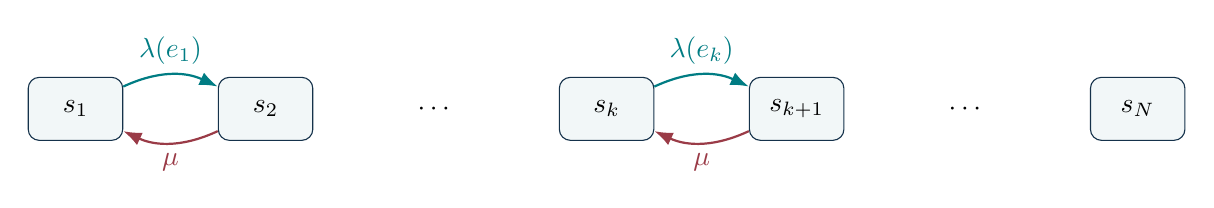
\begin{tikzpicture}[>=Latex,node distance=12mm,
state/.style={draw=navy,rounded corners,fill=pale,minimum width=12mm,minimum height=8mm},
up/.style={->,bend left=25,thick,teal},
down/.style={->,bend left=25,thick,rose}]
\node[state] (s1) {$s_1$};
\node[state,right=of s1] (s2) {$s_2$};
\node[right=of s2] (dots) {$\cdots$};
\node[state,right=of dots] (sk) {$s_k$};
\node[state,right=of sk] (skp) {$s_{k+1}$};
\node[right=of skp] (dots2) {$\cdots$};
\node[state,right=of dots2] (sn) {$s_N$};
\draw[up] (s1) to node[above] {$\lambda(e_1)$} (s2);
\draw[down] (s2) to node[below] {$\mu$} (s1);
\draw[up] (sk) to node[above] {$\lambda(e_k)$} (skp);
\draw[down] (skp) to node[below] {$\mu$} (sk);
\end{tikzpicture}
\end{center}
At an interior state $s_k$, there are two possible moves:
\begin{itemize}
  \item an upward move $s_k\to s_{k+1}$, representing skill improvement, at rate
  $\lambda(e_k(a))$;
  \item a downward move $s_k\to s_{k-1}$, representing skill depreciation or forgetting, at rate $\mu$.
\end{itemize}
The model therefore specifies
\[
  K_{s_k,s_{k+1}}(a)=\lambda(e_k(a)),
  \qquad K_{s_k,s_{k-1}}(a)=\mu,
\]
where $\lambda>0$ is increasing, concave, and differentiable, and $\mu>0$ is skill decay.  The symbol
$K_{s_i,s_j}$ records the off-diagonal transition rate from $s_i$ to $s_j$; it is not a transition
probability.  The assumptions on $\lambda$ have a direct economic meaning:
\begin{itemize}
  \item $\lambda(e)>0$: upward learning remains possible at every effort level;
  \item $\lambda'(e)\ge0$: more effort makes skill improvement arrive faster;
  \item $\lambda''(e)\le0$: the learning-rate gain from another unit of effort is diminishing.
\end{itemize}

Over a short interval $h$, conditional on currently being at an interior state $s_k$,
\begin{align*}
\Pp(\text{move up during }[t,t+h])
  &=\lambda(e_k(a))h+o(h),\\
\Pp(\text{move down during }[t,t+h])
  &=\mu h+o(h),\\
\Pp(\text{remain at }s_k\text{ during }[t,t+h])
  &=1-[\lambda(e_k(a))+\mu]h+o(h).
\end{align*}
The probability of two or more moves during such a short interval is $o(h)$.  At the lowest state $s_1$
there is no downward move, and at the highest state $s_N$ there is no upward move.

\paragraph{Waiting time and the direction of the next move.}
While the agent remains at $s_k$, the two rates act like competing exponential clocks.  Let
$\lambda_k=\lambda(e_k(a))$.  At an interior state:
\begin{itemize}
  \item the total rate at which \emph{some} skill change occurs is $\lambda_k+\mu$;
  \item the waiting time until the next change is exponential with mean $1/(\lambda_k+\mu)$;
  \item conditional on a change occurring next, it is upward with probability
  $\lambda_k/(\lambda_k+\mu)$ and downward with probability $\mu/(\lambda_k+\mu)$.
\end{itemize}
These last two fractions are probabilities because they divide each rate by the total rate.

\begin{example}[Interpreting annual skill-transition rates]
Suppose $\lambda_k=0.30$ per year and $\mu=0.10$ per year.  Then the total rate is $0.40$ per year, so the
expected waiting time until the next skill change is $1/0.40=2.5$ years.  Conditional on the next change,
\[
\Pp(\text{up next})=\frac{0.30}{0.40}=0.75,
\qquad
\Pp(\text{down next})=\frac{0.10}{0.40}=0.25.
\]
For one month, $h=1/12$ year, the short-interval approximations are
\[
\Pp(\text{up})\approx0.30/12=0.025,
\quad
\Pp(\text{down})\approx0.10/12=0.0083,
\quad
\Pp(\text{stay})\approx0.9667.
\]
\end{example}

\paragraph{Connection to the generator matrix.}
If states are indexed by $k=1,\ldots,N$, the continuous-time Markov generator $Q$ has, at an interior
state,
\[
Q_{k,k+1}=\lambda_k,
\qquad Q_{k,k-1}=\mu,
\qquad Q_{k,k}=-(\lambda_k+\mu).
\]
All other entries in row $k$ are zero, and the row sums to zero.  The negative diagonal entry is not a
negative probability; it is a bookkeeping term that makes the forward equations work.  The stationary
condition used below is $\pi Q=0$.

\paragraph{Step 1: define the stationary distribution.}
Fix the AI level $a$.  A stationary probability $\pi_k(a)$ is the long-run probability of finding an agent
at skill state $s_k$.  Equivalently, it is the long-run fraction of time the skill process spends at $s_k$.
The probabilities must satisfy
\[
  \pi_k(a)\ge0,
  \qquad
  \sum_{k=1}^N\pi_k(a)=1.
\]
Stationarity means that these probabilities do not change over time: at each state, the probability mass
flowing in per unit of time equals the probability mass flowing out.

\paragraph{Step 2: write detailed balance across one edge.}
For compact notation, define
\[
  \lambda_k(a):=\lambda(e_k(a)).
\]
Consider the edge connecting neighboring states $s_k$ and $s_{k+1}$.  In stationarity:
\begin{itemize}
  \item the mass at $s_k$ is $\pi_k(a)$ and each unit of that mass moves upward at rate $\lambda_k(a)$,
  so the upward flow is $\pi_k(a)\lambda_k(a)$;
  \item the mass at $s_{k+1}$ is $\pi_{k+1}(a)$ and each unit moves downward at rate $\mu$, so the
  downward flow is $\pi_{k+1}(a)\mu$.
\end{itemize}
Detailed balance equates these two opposite flows:
\begin{equation}
  \boxed{\pi_k(a)\lambda_k(a)=\pi_{k+1}(a)\mu.}
  \label{eq:edge-detailed-balance}
\end{equation}
Both sides have units of probability mass per unit of time.  Since $\mu>0$, divide by $\mu$ to obtain the
adjacent-probability recursion
\begin{equation}
  \boxed{\pi_{k+1}(a)=\pi_k(a)\frac{\lambda_k(a)}{\mu}.}
  \label{eq:stationary-recursion}
\end{equation}
This equation says that the stationary mass rises from $s_k$ to $s_{k+1}$ when the upward rate exceeds the
downward rate, and falls when the upward rate is smaller:
\[
  \frac{\pi_{k+1}(a)}{\pi_k(a)}
  =\frac{\lambda_k(a)}{\mu}.
\]

\paragraph{Step 3: apply the recursion repeatedly.}
Starting from $\pi_1(a)$, equation \eqref{eq:stationary-recursion} gives
\begin{align*}
\pi_2(a)
&=\pi_1(a)\frac{\lambda_1(a)}{\mu},\\
\pi_3(a)
&=\pi_2(a)\frac{\lambda_2(a)}{\mu}
=\pi_1(a)\frac{\lambda_1(a)}{\mu}\frac{\lambda_2(a)}{\mu},\\
\pi_4(a)
&=\pi_3(a)\frac{\lambda_3(a)}{\mu}
=\pi_1(a)\frac{\lambda_1(a)}{\mu}
             \frac{\lambda_2(a)}{\mu}
             \frac{\lambda_3(a)}{\mu}.
\end{align*}
The pattern is now visible.  To reach state $s_k$ from the reference state $s_1$, we multiply the
upward-to-downward rate ratio along every intervening edge:
\begin{equation}
  \boxed{
  \pi_k(a)=\pi_1(a)\prod_{i=1}^{k-1}\frac{\lambda_i(a)}{\mu}
  =\pi_1(a)\prod_{i=1}^{k-1}\frac{\lambda(e_i(a))}{\mu}.}
  \label{eq:stationary-product-form}
\end{equation}
The product symbol means
\[
  \prod_{i=1}^{k-1}\frac{\lambda_i(a)}{\mu}
  =\frac{\lambda_1(a)}{\mu}\frac{\lambda_2(a)}{\mu}\cdots
   \frac{\lambda_{k-1}(a)}{\mu}.
\]
For $k=1$, there are no factors to multiply.  By convention, this \emph{empty product} equals one, so
\eqref{eq:stationary-product-form} also returns $\pi_1(a)$ correctly.

\paragraph{Step 4: determine $\pi_1(a)$ by normalization.}
The recursion determines every probability relative to $\pi_1(a)$, but we still need their common scale.
Use the fact that probabilities sum to one:
\begin{align*}
1
&=\sum_{k=1}^N\pi_k(a)\\
&=\pi_1(a)+\sum_{k=2}^N
\pi_1(a)\prod_{i=1}^{k-1}\frac{\lambda(e_i(a))}{\mu}\\
&=\pi_1(a)\left[
1+\sum_{k=2}^N\prod_{i=1}^{k-1}\frac{\lambda(e_i(a))}{\mu}
\right].
\end{align*}
Dividing by the expression in square brackets gives
\begin{equation}
  \boxed{
  \pi_1(a)=\left(
  1+\sum_{k=2}^N\prod_{i=1}^{k-1}\frac{\lambda(e_i(a))}{\mu}
  \right)^{-1}.}
  \label{eq:stationary-normalizer}
\end{equation}
The exponent $-1$ means ``take the reciprocal'': $z^{-1}=1/z$.  It appears because the bracketed term is
the normalization constant required to make all probabilities sum to one.

\paragraph{Step 5: take probability-weighted averages.}
At state $s_k$, the agent exerts effort $e_k(a)$ and produces $p^\star(s_k,a)$.  Since the stationary
probability of that state is $\pi_k(a)$, the law of total expectation gives
\begin{align*}
\calE(a)
&=\E[\text{effort in stationarity}]
=\sum_{k=1}^N\pi_k(a)e_k(a),\\
\calP(a)
&=\E[\text{productivity in stationarity}]
=\sum_{k=1}^N\pi_k(a)p^\star(s_k,a).
\end{align*}
These are ordinary weighted averages: each state-specific outcome is multiplied by the long-run fraction of
time spent in that state.

\begin{example}[A two-state stationary distribution]
Suppose $N=2$, the upward rate is $\lambda_1=0.30$ per year, and the downward rate is $\mu=0.10$ per
year.  Detailed balance gives
\[
  \pi_1(0.30)=\pi_2(0.10)
  \quad\Longrightarrow\quad
  \pi_2=3\pi_1.
\]
Together with $\pi_1+\pi_2=1$, this gives $4\pi_1=1$, hence
\[
  \pi_1=0.25,
  \qquad
  \pi_2=0.75.
\]
The process spends $25\%$ of the long run in the low-skill state and $75\%$ in the high-skill state.  If
effort is $2$ in state 1 and $0.5$ in state 2, stationary effort is
\[
  \calE=0.25(2)+0.75(0.5)=0.875.
\]
If the two productivity levels are $10$ and $16$, stationary productivity is
\[
  \calP=0.25(10)+0.75(16)=14.5.
\]
\end{example}

The derivation above proves the following proposition.
\begin{proposition}[Stationary skill distribution]
\begin{align*}
  \pi_k(a)&=\pi_1(a)\prod_{i=1}^{k-1}\frac{\lambda(e_i(a))}{\mu},\\
  \pi_1(a)&=\left(1+\sum_{k=2}^{N}\prod_{i=1}^{k-1}
             \frac{\lambda(e_i(a))}{\mu}\right)^{-1}.
\end{align*}
The stationary effort and productivity are
\[
  \calE(a)=\sum_{k=1}^N\pi_k(a)e_k(a),
  \qquad
  \calP(a)=\sum_{k=1}^N\pi_k(a)p^\star(s_k,a).
\]
\end{proposition}

\subsection{Why edge-by-edge detailed balance solves stationarity}

It remains to verify that balancing each neighboring edge really solves the full stationarity equation
$\pi Q=0$.  At an interior state $s_k$, the inflow comes from $s_{k-1}$ and $s_{k+1}$, while the outflow
goes to those same two states.  Therefore the $k$th stationarity equation is
\[
\pi_{k-1}\lambda_{k-1}+\pi_{k+1}\mu-\pi_k(\lambda_k+\mu)=0.
\]
Detailed balance on the lower and upper edges gives, respectively,
\[
  \pi_{k-1}\lambda_{k-1}=\pi_k\mu,
  \qquad
  \pi_{k+1}\mu=\pi_k\lambda_k.
\]
Substituting these two equalities into the left side of the stationarity equation yields
\[
  \pi_k\mu+\pi_k\lambda_k-\pi_k(\lambda_k+\mu)=0.
\]
Thus inflow equals outflow at every interior state.  At $s_1$, the only balance equation is
$\pi_1\lambda_1=\pi_2\mu$; at $s_N$, it is
$\pi_{N-1}\lambda_{N-1}=\pi_N\mu$.  Hence the boundary equations also hold.  Positivity of all admissible
rates makes the finite chain irreducible, so the normalized stationary distribution is unique.

\subsection{Activity regimes}

The positive-part formula from Section~3 gives, at every skill state,
\[
  e_k(a)=\pos{x^\star-s_k-a}.
\]
Before introducing the intervals used in the paper, let us translate this formula into a threshold rule.
By the definition of the positive part,
\begin{align*}
e_k(a)>0
&\iff x^\star-s_k-a>0\\
&\iff a<x^\star-s_k\\
&\iff s_k+a<x^\star.
\end{align*}
Thus, state $s_k$ is \emph{active} when skill plus AI has not yet reached the preferred total input
$x^\star$.  It is \emph{inactive} when $s_k+a\ge x^\star$, because then optimal effort is zero.

Because $s_1\le s_2\le\cdots\le s_N$, the effort thresholds satisfy
\[
  x^\star-s_1\ge x^\star-s_2\ge\cdots\ge x^\star-s_N.
\]
As $a$ rises, high-skill states therefore stop exerting effort first.  The active states always form a
lower block $\{1,\ldots,m\}$; one cannot have state $s_k$ inactive while a higher state $s_{k+1}$ is
active.

\paragraph{Constructing the interval $I_m$ step by step.}
Suppose exactly the first $m$ states are active.  Then state $m$ must still exert effort, while state
$m+1$ must already exert zero effort:
\[
  a<x^\star-s_m,
  \qquad
  a\ge x^\star-s_{m+1}.
\]
Ignoring the endpoint convention for one moment, this places $a$ between the two neighboring thresholds.
The paper uses
\[
  I_m=\bigl(\pos{x^\star-s_{m+1}},\pos{x^\star-s_m}\bigr],
  \qquad m=1,\ldots,N-1,
\]
together with
\[
  I_0=[\pos{x^\star-s_1},\infty),
  \qquad
  I_N=[0,\pos{x^\star-s_N}].
\]
The notation $I_m$ should be read as ``the region with $m$ active states.''  The positive parts are needed
because the admissible AI level satisfies $a\ge0$; a negative effort threshold lies outside the domain.
At a shared endpoint, one state's optimal effort is exactly zero.  Assigning that endpoint to either
neighboring interval does not change any value, although it can change which one-sided derivative is used.

For $a$ in the interior of $I_m$,
\[
\begin{aligned}
k\le m:\quad
&e_k(a)=x^\star-s_k-a>0,\quad
s_k+e_k(a)+a=x^\star,\quad
p_k^\star(a)=p(x^\star),\\
k\ge m+1:\quad
&e_k(a)=0,\quad
s_k+e_k(a)+a=s_k+a,\quad
p_k^\star(a)=p(s_k+a).
\end{aligned}
\]
Consequently, inside one regime,
\[
e_k'(a)=
\begin{cases}-1,&k\le m,\\0,&k\ge m+1,\end{cases}
\qquad
\frac{d}{da}p_k^\star(a)=
\begin{cases}0,&k\le m,\\p'(s_k+a),&k\ge m+1.\end{cases}
\]
This is why the regime partition is useful: all formulas are smooth in the interior of $I_m$, and the only
formula changes occur when a state reaches zero effort.

\begin{example}[Locating the activity regimes]
Let $x^\star=10$ and $(s_1,s_2,s_3)=(2,6,9)$.  The three effort thresholds are
\[
  x^\star-s_1=8,
  \qquad x^\star-s_2=4,
  \qquad x^\star-s_3=1.
\]
Hence
\[
I_3=[0,1],\qquad I_2=(1,4],\qquad I_1=(4,8],\qquad I_0=[8,\infty).
\]
For example, at $a=3\in I_2$,
\[
e_1=10-2-3=5,\qquad e_2=10-6-3=1,\qquad e_3=0.
\]
Exactly two states are active, as the subscript of $I_2$ indicates.
\end{example}

\subsection{The sensitivity gap}

The theorem compares two effects of a marginal increase in AI near the right endpoint of $I_m$.  Write
\[
  a_m:=x^\star-s_m,
  \qquad
  d_m:=s_{m+1}-s_m>0.
\]
At $a=a_m$, state $s_m$ has just reached zero effort.  For every active state $j\le m$,
\[
e_j(a_m)
=x^\star-s_j-(x^\star-s_m)
=s_m-s_j.
\]
The first inactive state has total input
\[
  s_{m+1}+a_m=x^\star+s_{m+1}-s_m=x^\star+d_m.
\]
These two substitutions explain every argument appearing in the definition below.

For $m\in\{1,\ldots,N-1\}$, define
\begin{equation}
\boxed{
\Delta_m=
\underbrace{\sum_{j=1}^m\frac{\lambda'(s_m-s_j)}{\lambda(s_m-s_j)}}_{
\text{relative sensitivity of learning}}
-
\underbrace{\frac{p'(x^\star+d_m)}
{p(x^\star+d_m)-p(x^\star)}}_{
\text{relative sensitivity of the productivity premium}}.}
\label{eq:sensitivity-gap}
\end{equation}

\paragraph{Why the ratios are called semi-elasticities.}
For any positive differentiable function $f$,
\[
  \frac{f'(x)}{f(x)}=\frac{d}{dx}\log f(x).
\]
It measures the proportional change in $f$ caused by a one-unit change in $x$.  It is called a
\emph{semi-elasticity} because the change in the denominator variable is measured in levels, not percentages.

To see the first term directly, consider the reciprocal active-rate product
\[
 A_{1,m}(a)=\left[\prod_{j=1}^m\lambda(x^\star-s_j-a)\right]^{-1}.
\]
Taking logarithms converts the product into a sum:
\[
 \log A_{1,m}(a)=-\sum_{j=1}^m\log\lambda(x^\star-s_j-a).
\]
Differentiate.  The outer minus sign and the derivative of $x^\star-s_j-a$, which is $-1$, cancel:
\begin{align*}
\frac{A_{1,m}'(a)}{A_{1,m}(a)}
&=\frac{d}{da}\log A_{1,m}(a)\\
&=\sum_{j=1}^m
\frac{\lambda'(x^\star-s_j-a)}{\lambda(x^\star-s_j-a)}.
\end{align*}
Evaluating at $a=a_m$ gives the first term of $\Delta_m$.

For the direct-gain channel, define the productivity premium of the first inactive state by
\[
  R_m(a):=p(s_{m+1}+a)-p(x^\star)>0.
\]
Since $p(x^\star)$ is constant,
\[
  R_m'(a)=p'(s_{m+1}+a),
  \qquad
  \frac{R_m'(a)}{R_m(a)}
  =\frac{p'(s_{m+1}+a)}{p(s_{m+1}+a)-p(x^\star)}.
\]
At $a=a_m$, this is precisely the second term of $\Delta_m$.

Therefore $\Delta_m>0$ means that, at the regime endpoint, the learning-weight channel changes
proportionally faster than the direct productivity premium.  It does \emph{not} by itself say that
$\calP'(a)<0$: the decay rate $\mu$ also determines how strongly those local sensitivities enter the
stationary distribution.  Section~4.8 makes that additional step explicit.

\begin{example}[Reading the sign of the sensitivity gap]
Take $m=1$, $\lambda(e)=1+e$, $p(x)=\log(1+x)$, $x^\star=3$, $s_1=0$, and $s_2=2$.
Then $d_1=2$, and
\[
\frac{\lambda'(0)}{\lambda(0)}=1,
\qquad
\frac{p'(5)}{p(5)-p(3)}
=\frac{1/6}{\log(6)-\log(4)}
\approx0.411.
\]
Thus $\Delta_1\approx1-0.411=0.589>0$.  In this example the learning channel is locally more sensitive,
so a productivity-decline region becomes possible when skill decay is sufficiently large.
\end{example}

\subsection{A complete proof of skill degradation}

Let $a_\ell<a_h$, where the subscripts mean ``low AI'' and ``high AI.''  We will prove carefully that
the low-AI skill distribution places relatively more probability on high skill.

\paragraph{Step 1: compare effort state by state.}
The deterministic optimizer is
\[
e_i(a)=\pos{x^\star-s_i-a}.
\]
Increasing $a$ weakly reduces the expression inside the positive part.  Hence
\[
  e_i(a_\ell)\ge e_i(a_h)
  \qquad\text{for every }i.
\]
Because $\lambda$ is increasing and $\mu>0$ is unchanged,
\begin{equation}
  r_i^\ell:=\frac{\lambda(e_i(a_\ell))}{\mu}
  \ge
  r_i^h:=\frac{\lambda(e_i(a_h))}{\mu}.
  \label{eq:ratio-order}
\end{equation}
Recall that $r_i=\pi_{i+1}/\pi_i$.  Thus every adjacent high-to-low probability ratio is more favorable
to high skill under low AI.

\paragraph{Step 2: remove the normalizing constants.}
For either AI level $q\in\{\ell,h\}$, define
\[
  w_1^q:=1,
  \qquad
  w_k^q:=\prod_{i=1}^{k-1}r_i^q\quad(k\ge2),
  \qquad
  T^q:=\sum_{j=1}^N w_j^q.
\]
The stationary probabilities are simply
\[
  \pi_k(a_q)=\frac{w_k^q}{T^q}.
\]
Therefore the probability of being in one of the lowest $k$ states is
\[
  F^q(k):=\sum_{j=1}^k\pi_j(a_q)
  =\frac{\sum_{j=1}^k w_j^q}{T^q}.
\]
First-order stochastic dominance of the low-AI distribution means
\[
  F^\ell(k)\le F^h(k)
  \quad\text{for every }k.
\]
The inequality points this way because a smaller lower-tail probability means less mass on low skill and
more mass on high skill.

\paragraph{Step 3: cross-multiply and identify what must be compared.}
All weights are positive, so both denominators are positive.  Thus
\begin{align*}
F^\ell(k)\le F^h(k)
\quad\Longleftrightarrow\quad
\left(\sum_{j=1}^k w_j^\ell\right)
\left(\sum_{n=1}^N w_n^h\right)
\le
\left(\sum_{j=1}^k w_j^h\right)
\left(\sum_{n=1}^N w_n^\ell\right).
\end{align*}
Expand both products.  The terms with both indices in the lower block, $j\le k$ and $n\le k$, are the
same after interchanging the dummy indices $j$ and $n$, so their double sums cancel.  It remains to compare
the cross-block terms $j\le k<n$.  For each such pair we need
\begin{equation}
  w_j^\ell w_n^h\le w_j^h w_n^\ell.
  \label{eq:cross-weight}
\end{equation}

\paragraph{Step 4: prove every cross-block comparison.}
Since $n>j$, all factors before state $j$ cancel in the ratio:
\begin{align*}
\frac{w_n^\ell}{w_j^\ell}
&=\frac{\prod_{i=1}^{n-1}r_i^\ell}
        {\prod_{i=1}^{j-1}r_i^\ell}
=\prod_{i=j}^{n-1}r_i^\ell\\
&\ge\prod_{i=j}^{n-1}r_i^h
=\frac{w_n^h}{w_j^h},
\end{align*}
where the inequality uses \eqref{eq:ratio-order} factor by factor.  Multiplying by the positive number
$w_j^\ell w_j^h$ gives \eqref{eq:cross-weight}.  Summing over every pair $j\le k<n$ proves
$F^\ell(k)\le F^h(k)$.

\begin{proposition}[Skill degradation]
The low-assistance stationary distribution first-order stochastically dominates the high-assistance one:
\[
  \sum_{i=1}^k\pi_i(a_\ell)\le\sum_{i=1}^k\pi_i(a_h),\qquad k=1,\ldots,N.
\]
\end{proposition}

\begin{intuition}
At every current skill, more AI reduces effort.  This lowers every upward transition rate without changing
the decay rate.  Stationary mass therefore shifts toward low skill.  This is the distributional ingredient of
the Simpson-type reversal.
\end{intuition}

\begin{example}[A three-state dominance calculation]
Suppose the adjacent ratios are
\[
(r_1^\ell,r_2^\ell)=(2,1.5),
\qquad
(r_1^h,r_2^h)=(1,0.75).
\]
The unnormalized weights are
\[
(w_1^\ell,w_2^\ell,w_3^\ell)=(1,2,3),
\qquad
(w_1^h,w_2^h,w_3^h)=(1,1,0.75).
\]
After normalization,
\[
\pi(a_\ell)=\left(\frac16,\frac13,\frac12\right),
\qquad
\pi(a_h)=\left(\frac4{11},\frac4{11},\frac3{11}\right).
\]
The lower-tail probabilities are
\[
F^\ell(1)=\frac16<\frac4{11}=F^h(1),
\qquad
F^\ell(2)=\frac12<\frac8{11}=F^h(2).
\]
Thus high AI shifts stationary probability toward the lower states even though it may raise productivity
conditional on any fixed state.
\end{example}

\subsection{Rewriting stationary productivity on one regime}

Fix an interior regime $I_m$, where $1\le m\le N-1$.  The goal of this subsection is to transform the
stationary weighted average into a quotient whose derivative separates the direct AI gain from the
endogenous deskilling loss.

\paragraph{Step 1: write unnormalized stationary weights.}
Define
\[
  q_1(a):=1,
  \qquad
  q_k(a):=\prod_{i=1}^{k-1}\frac{\lambda(e_i(a))}{\mu}
  \quad(k\ge2).
\]
Then
\[
  \pi_k(a)=\frac{q_k(a)}{\sum_{j=1}^Nq_j(a)},
  \qquad
  \calP(a)=
  \frac{\sum_{k=1}^Nq_k(a)p_k^\star(a)}
       {\sum_{k=1}^Nq_k(a)}.
\]
This is just the stationary formula with the common normalization constant canceled from numerator and
denominator.

Inside $I_m$, states $1,\ldots,m$ are active and states $m+1,\ldots,N$ are inactive.  Therefore
\[
  \lambda(e_i(a))=
  \begin{cases}
  \lambda(x^\star-s_i-a),&i\le m,\\
  \lambda(0),&i\ge m+1.
  \end{cases}
\]
For an active destination state $k\le m$, the path from state 1 to state $k$ contains only active rates:
\[
  q_k(a)=\frac{\prod_{i=1}^{k-1}\lambda(x^\star-s_i-a)}{\mu^{k-1}}.
\]
For an inactive destination state $k\ge m+1$, the path first crosses all $m$ active rates and then crosses
$k-m-1$ edges whose rate is $\lambda(0)$:
\[
  q_k(a)=
  \frac{\left[\prod_{i=1}^{m}\lambda(x^\star-s_i-a)\right]
  \lambda(0)^{k-m-1}}{\mu^{k-1}}.
\]

\paragraph{Step 2: split active and inactive productivity.}
The state-level productivity is $p(x^\star)$ in every active state and $p(s_k+a)$ in every inactive
state.  Hence
\begin{align*}
\calP(a)
=\frac{
p(x^\star)\sum_{k=1}^m q_k(a)
+\sum_{k=m+1}^Nq_k(a)p(s_k+a)}
{\sum_{k=1}^m q_k(a)+\sum_{k=m+1}^Nq_k(a)}.
\end{align*}
Let $Q(a)=\sum_{k=1}^Nq_k(a)$.  Add and subtract
$p(x^\star)\sum_{k=m+1}^Nq_k(a)$ in the numerator:
\begin{align*}
\calP(a)
&=\frac{p(x^\star)Q(a)
+\sum_{k=m+1}^Nq_k(a)[p(s_k+a)-p(x^\star)]}{Q(a)}\\
&=p(x^\star)+
\frac{\sum_{k=m+1}^Nq_k(a)[p(s_k+a)-p(x^\star)]}{Q(a)}.
\end{align*}
The bracket is the productivity premium of inactive state $k$ relative to the common active-state output.

\paragraph{Step 3: cancel the common active-rate product.}
Define the positive common factor
\[
  C_m(a):=\prod_{i=1}^m\lambda(x^\star-s_i-a).
\]
Divide every unnormalized weight by $C_m(a)$.  Multiplying all weights by the same positive number does not
change a weighted average.  For $k\le m$,
\begin{align*}
\frac{q_k(a)}{C_m(a)}
&=\frac{\prod_{i=1}^{k-1}\lambda(x^\star-s_i-a)}
{\mu^{k-1}\prod_{i=1}^{m}\lambda(x^\star-s_i-a)}\\
&=\frac{1}{\mu^{k-1}\prod_{i=k}^{m}\lambda(x^\star-s_i-a)}.
\end{align*}
The factors indexed $1,\ldots,k-1$ cancel, leaving only $k,\ldots,m$ in the denominator.  For $k\ge m+1$,
\[
  \frac{q_k(a)}{C_m(a)}
  =\frac{\lambda(0)^{k-m-1}}{\mu^{k-1}}.
\]
This motivates the abbreviations
\[
 A_{k,m}(a):=\left[\prod_{i=k}^{m}\lambda(x^\star-s_i-a)\right]^{-1},
 \qquad
 B_{k,m}:=\lambda(0)^{k-m-1}.
\]
Notice that $A_{k,m}$ depends on $a$, whereas $B_{k,m}$ does not.

Using these definitions,
\begin{equation}
\boxed{\calP(a)=p(x^\star)+\frac{N_m(a)}{D_m(a)},}
\label{eq:P-N-over-D}
\end{equation}
where
\begin{align*}
N_m(a)&=\sum_{k=m+1}^{N}\frac{B_{k,m}}{\mu^{k-1}}
       \bigl[p(s_k+a)-p(x^\star)\bigr],\\
D_m(a)&=\sum_{k=1}^{m}\frac{A_{k,m}(a)}{\mu^{k-1}}
       +\sum_{k=m+1}^{N}\frac{B_{k,m}}{\mu^{k-1}}.
\end{align*}
Every term in $D_m$ is positive, so $D_m(a)>0$.

\paragraph{Step 4: differentiate every component.}
Since the $B_{k,m}$ are constant in $a$,
\[
N_m'(a)=\sum_{k=m+1}^N
\frac{B_{k,m}}{\mu^{k-1}}p'(s_k+a).
\]
Only the $A_{k,m}$ terms in $D_m$ vary with $a$, so
\[
D_m'(a)=\sum_{k=1}^m\frac{A_{k,m}'(a)}{\mu^{k-1}}.
\]
For later use, logarithmic differentiation gives an explicit formula for each derivative:
\begin{align}
A_{k,m}'(a)
&=A_{k,m}(a)L_{k,m}(a),\nonumber\\
L_{k,m}(a)
&:=\sum_{j=k}^m
\frac{\lambda'(x^\star-s_j-a)}{\lambda(x^\star-s_j-a)}\ge0.
\label{eq:A-prime}
\end{align}

Apply the quotient rule $(N/D)'=(N'D-ND')/D^2$ to \eqref{eq:P-N-over-D}:
\begin{align}
\calP'(a)=\frac{1}{D_m(a)^2}\Bigg[&
\left(\sum_{k=m+1}^N\frac{B_{k,m}}{\mu^{k-1}}p'(s_k+a)\right)D_m(a)\nonumber\\
&-N_m(a)\left(\sum_{k=1}^m\frac{A'_{k,m}(a)}{\mu^{k-1}}\right)\Bigg].
\label{eq:Pprime}
\end{align}
The denominator is positive and therefore never affects the sign.  In the numerator:
\begin{itemize}
  \item the first term is the direct increase in the productivity of inactive states;
  \item the second term is the loss from changing stationary weights, because higher AI lowers active-state
  effort and therefore the upward transition rates.
\end{itemize}

\subsection{Why the derivative crosses zero at most once}

Equation~\eqref{eq:Pprime} appears complicated, but its sign can be written as ``a decreasing benefit minus
an increasing loss.''  Define
\begin{align*}
U_m(a)&:=\sum_{k=m+1}^N\frac{B_{k,m}}{\mu^{k-1}}p'(s_k+a),\\
V_m(a)&:=\sum_{k=m+1}^N\frac{B_{k,m}}{\mu^{k-1}}
[p(s_k+a)-p(x^\star)],\\
h_m(a)&:=\frac{D_m'(a)}{D_m(a)}
=\frac{\sum_{k=1}^m A'_{k,m}(a)/\mu^{k-1}}
{\sum_{k=1}^m A_{k,m}(a)/\mu^{k-1}
+\sum_{k=m+1}^N B_{k,m}/\mu^{k-1}}.
\end{align*}
Since $D_m>0$, multiply \eqref{eq:Pprime} by $D_m$:
\begin{equation}
  D_m(a)\calP'(a)=U_m(a)-V_m(a)h_m(a)=:G_m(a).
  \label{eq:G-sign}
\end{equation}
Thus $G_m$ and $\calP'$ always have the same sign.

\paragraph{Step 1: establish the easy monotonicities.}
Concavity of $p$ means $p'$ is weakly decreasing.  Every coefficient in $U_m$ is positive and constant,
so $U_m(a)$ is weakly decreasing.  Monotonicity of $p$ means every premium
$p(s_k+a)-p(x^\star)$ is weakly increasing, so $V_m(a)$ is weakly increasing.  It remains to show that
$h_m(a)$ is also weakly increasing.

\paragraph{Step 2: rewrite $h_m$ compactly.}
Put
\[
\bar A_k(a):=\frac{A_{k,m}(a)}{\mu^{k-1}},
\qquad
\bar B:=\sum_{k=m+1}^N\frac{B_{k,m}}{\mu^{k-1}},
\qquad
S(a):=\sum_{k=1}^m\bar A_k(a).
\]
Then $D_m=S+\bar B$, $D_m'=S'$, and
\[
  h_m(a)=\frac{S'(a)}{S(a)+\bar B}.
\]
From \eqref{eq:A-prime}, with $L_k=L_{k,m}(a)$,
\[
  \bar A_k'(a)=\bar A_k(a)L_k(a).
\]

\paragraph{Step 3: compute the second derivative of each $\bar A_k$.}
For a single summand in $L_k$, let $y_j(a)=x^\star-s_j-a$.  Since $y_j'(a)=-1$,
\begin{align*}
\frac{d}{da}\left(\frac{\lambda'(y_j)}{\lambda(y_j)}\right)
&=-\frac{\lambda''(y_j)\lambda(y_j)-[\lambda'(y_j)]^2}{\lambda(y_j)^2}\\
&=\frac{[\lambda'(y_j)]^2-\lambda''(y_j)\lambda(y_j)}{\lambda(y_j)^2}\ge0.
\end{align*}
The last inequality uses $\lambda>0$ and concavity, $\lambda''\le0$.  Applying the product rule to
$\bar A_k'=\bar A_kL_k$ gives
\begin{align}
\bar A_k''
&=\bar A_kL_k^2
+\bar A_k\sum_{j=k}^m
\frac{(\lambda')^2-\lambda''\lambda}{\lambda^2}
\ge \bar A_kL_k^2.
\label{eq:A-second-lower-bound}
\end{align}
Every unlabelled $\lambda$, $\lambda'$, and $\lambda''$ in the sum is evaluated at
$x^\star-s_j-a$.

\paragraph{Step 4: differentiate $h_m$.}
The quotient rule gives
\[
h_m'(a)=
\frac{S''(a)[S(a)+\bar B]-[S'(a)]^2}{[S(a)+\bar B]^2}.
\]
The denominator is positive.  For the numerator, first use $\bar B\ge0$ and
\eqref{eq:A-second-lower-bound}:
\begin{align*}
S''(S+\bar B)
&\ge S''S\\
&\ge
\left(\sum_{k=1}^m\bar A_kL_k^2\right)
\left(\sum_{k=1}^m\bar A_k\right).
\end{align*}
Weighted Cauchy--Schwarz says
\[
\left(\sum_{k=1}^m\bar A_kL_k\right)^2
\le
\left(\sum_{k=1}^m\bar A_k\right)
\left(\sum_{k=1}^m\bar A_kL_k^2\right).
\]
But $S'=\sum_k\bar A_kL_k$.  Therefore $S''(S+\bar B)\ge(S')^2$, so $h_m'(a)\ge0$.

\paragraph{Step 5: conclude the one-crossing result.}
We now know that $U_m$ decreases, while $V_m$ and $h_m$ are nonnegative and increase.  Their product
$V_mh_m$ therefore increases.  Consequently,
\[
  G_m(a)=U_m(a)-V_m(a)h_m(a)
\]
is weakly decreasing.  A decreasing function can cross zero at most once, and if it crosses, it can only
move from positive to negative.  Because $D_m>0$, the same statement applies to $\calP'(a)$.

\begin{lemma}[Within-regime shape]
On $I_m$, stationary productivity is either increasing everywhere or increasing and then decreasing.  A
decreasing subregion exists exactly when the left derivative at the right endpoint is negative.
\end{lemma}

The phrase ``left derivative at the right endpoint'' is important.  The derivative formula above applies
inside $I_m$.  At the right endpoint, state $m$ reaches zero effort and the formula changes in the next
regime, so we approach the endpoint from within $I_m$.  The shape lemma also establishes that the entry
derivative at the left boundary is nonnegative.  Combined with the one-crossing result, a negative exit
derivative is both necessary and sufficient for an interior maximum.

\subsection{The large-decay asymptotic and Theorem 1}

We now connect the endpoint derivative to the sensitivity gap.  Fix an intermediate regime and let
\[
  a_m=x^\star-s_m,
  \qquad z:=\frac1\mu.
\]
Large memory decay means large $\mu$, which is the same as small positive $z$.

\paragraph{Step 1: isolate the numerator determining the sign.}
At $a=a_m$, let $X_m(z)$ denote the square-bracketed numerator in \eqref{eq:Pprime}.  Using the notation
from Section~4.7,
\[
X_m(z)=U_m(a_m)D_m(a_m)-V_m(a_m)D_m'(a_m).
\]
Every occurrence of $1/\mu^{k-1}$ is $z^{k-1}$.  Since all sums are finite, $X_m(z)$ is a polynomial in
$z$.

\paragraph{Step 2: find the smallest power of $z$.}
In $U_m$ and $V_m$, the smallest state index is $k=m+1$, so their lowest power is
$z^{(m+1)-1}=z^m$.  In $D_m$ and $D_m'$, the smallest active index is $k=1$, so their lowest power is
$z^{1-1}=1$.  Therefore the lowest possible order in both products $U_mD_m$ and $V_mD_m'$ is $z^m$.
Only the pairing
\[
  \text{first inactive state }k=m+1
  \quad\text{with}\quad
  \text{lowest active index }k=1
\]
contributes to that coefficient.  All other pairings contain at least one additional factor of $z$.

Since $B_{m+1,m}=\lambda(0)^0=1$, the coefficient on $z^m$ is
\begin{align*}
c_m
&=p'(s_{m+1}+a_m)A_{1,m}(a_m)\\
&\quad-[p(s_{m+1}+a_m)-p(x^\star)]A_{1,m}'(a_m).
\end{align*}

\paragraph{Step 3: evaluate the endpoint arguments.}
At $a_m=x^\star-s_m$,
\[
s_{m+1}+a_m=x^\star+s_{m+1}-s_m,
\]
and
\[
A_{1,m}(a_m)
=\frac{1}{\prod_{i=1}^m\lambda(s_m-s_i)}.
\]
Equation~\eqref{eq:A-prime} also gives
\[
\frac{A_{1,m}'(a_m)}{A_{1,m}(a_m)}
=\sum_{j=1}^m\frac{\lambda'(s_m-s_j)}{\lambda(s_m-s_j)}.
\]
Substitute these expressions into $c_m$ and factor out the positive terms:
\begin{align*}
c_m
&=\frac{1}{\prod_{i=1}^m\lambda(s_m-s_i)}
\Bigg[p'(x^\star+s_{m+1}-s_m)\\
&\qquad-\bigl(p(x^\star+s_{m+1}-s_m)-p(x^\star)\bigr)
\sum_{j=1}^m\frac{\lambda'(s_m-s_j)}{\lambda(s_m-s_j)}\Bigg]\\
&=-C_m\Delta_m,
\end{align*}
where
\[
C_m:=\frac{p(x^\star+s_{m+1}-s_m)-p(x^\star)}
{\prod_{i=1}^m\lambda(s_m-s_i)}>0.
\]
The final equality follows by multiplying the definition of $\Delta_m$ by the positive productivity
premium and the positive reciprocal rate product.

\paragraph{Step 4: use the leading coefficient.}
We have shown
\[
  X_m(z)=(-C_m\Delta_m)z^m+\text{terms of order }z^{m+1}\text{ and higher}.
\]
For sufficiently small $z>0$, the first nonzero coefficient determines the sign of a polynomial.  Since
$z=1/\mu$, there is a finite threshold $\bar\mu_m$ such that, for $\mu>\bar\mu_m$,
\[
\operatorname{sgn}\calP'_{-}(a_m)
=\operatorname{sgn}X_m(1/\mu)
=-\operatorname{sgn}\Delta_m.
\]
If $\Delta_m=0$, the leading coefficient vanishes and higher-order terms must be examined; the theorem does
not claim a strict conclusion for that knife-edge case.

\begin{theorem}[Paper's Theorem 1]
There is $\bar\mu>0$ such that, for every $\mu>\bar\mu$ and nonempty $I_m$:
\begin{enumerate}
  \item if $1\le m\le N-1$ and $\Delta_m>0$, $\calP$ increases and then decreases on $I_m$;
  \item if $m\in\{0,N\}$ or $\Delta_m<0$, $\calP$ is weakly increasing on $I_m$.
\end{enumerate}
\end{theorem}

To obtain one threshold that works for every intermediate regime, take
\[
  \bar\mu:=\max_{m=1,\ldots,N-1}\bar\mu_m.
\]
There are only finitely many regimes, so this maximum is finite.  The within-regime one-crossing lemma then
turns the sign of the exit derivative into the claimed shape.

The two boundary regimes can be checked directly:
\begin{itemize}
  \item On $I_N$, every state is active.  Effort adjusts one for one to AI, total input stays at $x^\star$,
  and every state produces $p(x^\star)$.  Any weighted average of the same number is that number, so
  $\calP(a)=p(x^\star)$ is constant.
  \item On $I_0$, every state is inactive, so $e_k=0$ and every upward rate equals $\lambda(0)$.  The
  stationary probabilities are therefore independent of $a$, while each $p(s_k+a)$ is increasing.  Hence
  \[
  \calP'(a)=\sum_{k=1}^N\pi_k p'(s_k+a)\ge0.
  \]
\end{itemize}

Economically, large $\mu$ means that skill depreciates quickly.  The stationary distribution then reacts
strongly to whether current effort can rebuild skill.  Algebraically, the leading $z^m$ term isolates the
lowest active path and the first inactive state; the sign comparison for that marginal pair is exactly
$-\Delta_m$.

\subsection{Exact two-state calculation}

Let $N=2$ and $s_1<s_2$.  This case is useful because every step can be seen without summation notation.

\paragraph{Step 1: solve the stationary probabilities.}
There is one upward rate, $\lambda(e_1(a))$, and one downward rate, $\mu$.  Detailed balance and
normalization are
\[
  \pi_1\lambda(e_1)=\pi_2\mu,
  \qquad
  \pi_1+\pi_2=1.
\]
From the first equation, $\pi_2=\pi_1\lambda(e_1)/\mu$.  Substitute this into the second:
\[
  \pi_1\left(1+\frac{\lambda(e_1)}{\mu}\right)=1.
\]
Therefore
\begin{equation}
  \pi_1(a)=\frac{\mu}{\mu+\lambda(e_1(a))},
  \qquad
  \pi_2(a)=\frac{\lambda(e_1(a))}{\mu+\lambda(e_1(a))}.
  \label{eq:two-state-pi}
\end{equation}

\paragraph{Step 2: specialize to the intermediate regime.}
On $I_1=(x^\star-s_2,x^\star-s_1]$, state 1 is active and state 2 is inactive.  Thus
\[
e_1(a)=x^\star-s_1-a,
\qquad e_2(a)=0,
\]
and
\[
p_1^\star(a)=p(x^\star),
\qquad p_2^\star(a)=p(s_2+a).
\]
Define, for compactness,
\[
  L(a):=\lambda(x^\star-s_1-a),
  \qquad P_0:=p(x^\star),
  \qquad P_2(a):=p(s_2+a).
\]
Substituting \eqref{eq:two-state-pi} into the stationary weighted average gives
\begin{equation}
\boxed{
\calP(a)=\frac{\mu P_0+L(a)P_2(a)}{\mu+L(a)}.}
\label{eq:two-state-P}
\end{equation}

\paragraph{Step 3: differentiate without skipping the quotient-rule algebra.}
The derivatives of the moving pieces are
\[
L'(a)=-\lambda'(x^\star-s_1-a),
\qquad
P_2'(a)=p'(s_2+a).
\]
Apply the quotient rule to \eqref{eq:two-state-P}:
\begin{align*}
\calP'(a)
&=\frac{[L'P_2+LP_2'](\mu+L)-[\mu P_0+LP_2]L'}{(\mu+L)^2}\\
&=\frac{\mu L'P_2+LL'P_2+(\mu+L)LP_2'
-\mu P_0L'-LL'P_2}{(\mu+L)^2}\\
&=\frac{(\mu+L)LP_2'+\mu L'(P_2-P_0)}{(\mu+L)^2}\\
&=\frac{(\mu+L)Lp'(s_2+a)
-\mu\lambda'(x^\star-s_1-a)[p(s_2+a)-p(x^\star)]}{(\mu+L)^2}.
\end{align*}
The terms $LL'P_2$ cancel on the second line.  The remaining positive term is the direct gain in state 2;
the subtracted term is the loss from the falling probability $\pi_2(a)$ of occupying that high-skill state.

\paragraph{Step 4: show that the numerator falls with AI.}
As $a$ increases, effort $x^\star-s_1-a$ falls.  Since $\lambda$ is increasing,
$L(a)$ falls.  Concavity of $p$ makes $p'(s_2+a)$ fall.  Therefore the entire positive product
$(\mu+L)Lp'$ falls.  Meanwhile, concavity of $\lambda$ means $\lambda'(e)$ is decreasing in $e$; because
$e$ falls with $a$, $\lambda'(e)$ weakly rises.  The productivity premium
$p(s_2+a)-p(x^\star)$ also rises.  Hence the subtracted product weakly rises.  The numerator is therefore
decreasing in $a$ and can cross zero at most once.

\paragraph{Step 5: evaluate both endpoints.}
At the left endpoint $a_L=x^\star-s_2$, state 2 has total input $x^\star$, so its productivity premium is
zero.  Writing $d=s_2-s_1$,
\[
  L(a_L)=\lambda(d),
  \qquad
  \text{numerator at }a_L=(\mu+\lambda(d))\lambda(d)p'(x^\star)>0.
\]
Thus productivity initially rises as we enter $I_1$.

At the right endpoint $a_R=x^\star-s_1$, state 1's effort is zero.  Define
\[
  R:=p(x^\star+s_2-s_1)-p(x^\star)>0,
  \qquad
  p_R':=p'(x^\star+s_2-s_1).
\]
The endpoint numerator is
\begin{align*}
H_R
&=(\mu+\lambda(0))\lambda(0)p_R'-\mu\lambda'(0)R\\
&=\lambda(0)^2p_R'
-\mu\bigl[\lambda'(0)R-\lambda(0)p_R'\bigr].
\end{align*}
For $H_R<0$, the bracket must first be positive.  Dividing that requirement by the positive number
$\lambda(0)R$ gives
\[
  \frac{\lambda'(0)}{\lambda(0)}-\frac{p_R'}{R}>0,
\]
which is exactly $\Delta_1>0$.  Conditional on this, $H_R<0$ is equivalent to
\begin{equation}
\mu>
\bar\mu_2:=
\frac{\lambda(0)^2p_R'}
{\lambda'(0)R-\lambda(0)p_R'}.
\label{eq:two-state-mu-threshold}
\end{equation}

We therefore obtain the complete two-state classification:
\begin{itemize}
  \item if $\Delta_1>0$ and $\mu>\bar\mu_2$, $\calP$ first increases and then decreases on $I_1$;
  \item if either condition fails, $\calP$ is weakly increasing on $I_1$.
\end{itemize}
Together with a flat $I_2$ and an increasing $I_0$, the first case produces the paper's global
$N$-shaped profile: flat, then rising, then falling, and finally rising again.

\begin{example}[Computing the exact decay threshold]
Continue the earlier example $\lambda(e)=1+e$, $p(x)=\log(1+x)$, $x^\star=3$, $s_1=0$, and $s_2=2$.
Then
\[
R=\log(6)-\log(4)\approx0.4055,
\qquad p_R'=\frac16,
\]
so
\[
\bar\mu_2
=\frac{1/6}{0.4055-1/6}
\approx0.698.
\]
Thus $\mu=1$ lies above the threshold and yields an increasing-then-decreasing intermediate regime,
whereas $\mu=0.5$ does not.
\end{example}

\subsection{Why an arbitrarily large shortfall is possible}

The preceding theorem establishes that productivity can fall.  The next proposition is stronger: for any
target $\varepsilon>0$, primitives can be chosen so that productivity under higher AI is at most an
$\varepsilon$ fraction of productivity under lower AI.  This is an existence construction, not a claim
that every calibration has a large decline.

Assume $s_1=0<s_2<\cdots<s_N$.  It is enough to consider $0<\varepsilon\le1$, because a ratio below one
automatically satisfies any target $\varepsilon>1$.

\paragraph{Step 1: select two nearby AI levels.}
Choose a number $z$ satisfying
\[
  0<z\le\min\{x^\star,s_2\},
\]
and compare
\[
  a_h=x^\star,
  \qquad
  a_\ell=x^\star-z<a_h.
\]
At $a_h$, even the lowest state has $s_1+a_h=x^\star$, so every state exerts zero effort.  At $a_\ell$,
state 1 supplies exactly $z$ units of effort:
\[
  e_1(a_\ell)=x^\star-0-(x^\star-z)=z.
\]
For every $k\ge2$, $s_k\ge s_2\ge z$, so
\[
  e_k(a_\ell)=\pos{z-s_k}=0.
\]
Thus the small reduction in AI activates effort only at the lowest state.

\paragraph{Step 2: send the zero-effort learning rate toward zero.}
At $a_h$, all adjacent upward rates equal $\lambda(0)$.  If $\lambda(0)$ is very small relative to $\mu$,
the stationary ratios $\pi_{k+1}/\pi_k=\lambda(0)/\mu$ are very small, so almost all mass lies at $s_1$.
Consequently,
\[
  \calP(a_h)\longrightarrow p(x^\star)
  \qquad\text{as }\lambda(0)\to0.
\]

At $a_\ell$, the first upward rate is $\lambda(z)$ and all subsequent upward rates are $\lambda(0)$.
The unnormalized weights are
\[
1,\quad
\frac{\lambda(z)}{\mu},\quad
\frac{\lambda(z)}{\mu}\frac{\lambda(0)}{\mu},\quad\ldots.
\]
As $\lambda(0)\to0$, all weights beyond state 2 vanish.  The limiting probabilities on the first two states
are therefore
\[
  \pi_1\to\frac{1}{1+r},
  \qquad
  \pi_2\to\frac{r}{1+r},
  \qquad
  r:=\frac{\lambda(z)}{\mu}.
\]
State 1 produces $p(x^\star)$ because its effort fills the gap; state 2 produces
$p(s_2+a_\ell)=p(x^\star+s_2-z)$.  Hence
\begin{equation}
\frac{\calP(a_h)}{\calP(a_\ell)}
\longrightarrow
\frac{p(x^\star)}{
\dfrac{1}{1+r}\left[p(x^\star)+r\,p(x^\star+s_2-z)\right]}.
\label{eq:shortfall-limit}
\end{equation}

\paragraph{Step 3: make production almost linear.}
Choose a concave production function whose slopes just below and above $x^\star$ are arbitrarily close.
In the limiting linear calculation, multiplicative slope constants cancel from
\eqref{eq:shortfall-limit}.  Let
\[
  w:=\frac{r}{1+r}=\frac{\lambda(z)}{\mu+\lambda(z)}.
\]
The ratio becomes arbitrarily close to
\[
  \frac{x^\star}{(1-w)x^\star+w(x^\star+s_2-z)}.
\]
For fixed $z$, this fractional expression is minimized at the admissible boundary $x^\star=z$, giving
\[
  \frac{z}{(1-w)z+ws_2}.
\]

\paragraph{Step 4: choose the scale and learning probability.}
Set
\[
  z=x^\star=\frac{\varepsilon s_2}{4}
\]
and choose the concave learning technology so that
\[
  w=\frac{\lambda(z)}{\mu+\lambda(z)}\ge1-\frac{\varepsilon}{4}.
\]
Then
\[
\frac{z}{(1-w)z+ws_2}
\le\frac{z}{ws_2}
\le\frac{\varepsilon/4}{1-\varepsilon/4}
\le\varepsilon.
\]
The last inequality holds for $0<\varepsilon\le1$.  Taking the almost-linear approximation and
$\lambda(0)$ sufficiently close to their limiting values preserves the strict bound.

The order of construction matters: choose the nearly linear $p$ and its target $x^\star$, make
$\lambda(0)$ small so that zero effort cannot sustain skill, and then make $\lambda(z)/\mu$ large enough
that a small amount of effort moves most stationary mass to state 2.

\subsection{Simpson's paradox and the exogenous benchmark}

At a fixed skill state, AI never lowers productivity:
\[
  \frac{\partial p_k^\star(a)}{\partial a}\ge0.
\]
How, then, can the stationary average fall?  The answer is that both the within-state outcomes and the
weights depend on AI.

\paragraph{The derivative decomposition.}
Differentiate the weighted average using the product rule:
\begin{align}
\calP'(a)
&=\frac{d}{da}\sum_{k=1}^N\pi_k(a)p_k^\star(a)\nonumber\\
&=\underbrace{\sum_{k=1}^N\pi_k(a)
\frac{\partial p_k^\star(a)}{\partial a}}_{\text{within-state or direct effect}}
+\underbrace{\sum_{k=1}^N\pi_k'(a)p_k^\star(a)}_{\text{composition effect}}.
\label{eq:simpson-decomposition}
\end{align}
The first term is nonnegative.  Because probabilities always sum to one,
\[
  \sum_{k=1}^N\pi_k'(a)=\frac{d}{da}1=0.
\]
Therefore a common constant may be subtracted inside the composition term without changing it:
\[
  \sum_k\pi_k'p_k^\star
  =\sum_k\pi_k'[p_k^\star-c]
  \qquad\text{for any }c.
\]
This makes clear that only reallocations between states with different productivity matter.

For two states, use $\pi_1'=-\pi_2'$ to obtain
\begin{equation}
\calP'
=\pi_1(p_1^\star)'+\pi_2(p_2^\star)'
+\pi_2'(p_2^\star-p_1^\star).
\label{eq:two-state-simpson}
\end{equation}
Skill degradation implies $\pi_2'(a)\le0$, while normally $p_2^\star>p_1^\star$.  The last term is then
negative.  If its magnitude exceeds the first two nonnegative terms, aggregate productivity falls even
though productivity rises within both states.

\begin{example}[A numerical Simpson reversal]
Suppose the low-AI stationary weights are $(0.25,0.75)$ and state productivities are $(10,16)$, so
\[
  \calP_{\ell}=0.25(10)+0.75(16)=14.5.
\]
Under higher AI, suppose each state becomes one unit more productive, giving $(11,17)$, but deskilling
changes the weights to $(0.75,0.25)$.  Then
\[
  \calP_h=0.75(11)+0.25(17)=12.5<14.5.
\]
The within-state effect is positive in both groups; the aggregate falls only because much more probability
is assigned to the low-skill group.
\end{example}

\paragraph{Why exogenous transitions eliminate the paradox.}
If upward transition rates are fixed numbers $\lambda_k$ rather than functions of effort, the stationary
distribution is
\[
  \pi_k=\pi_1\prod_{i=1}^{k-1}\frac{\lambda_i}{\mu},
\]
which does not depend on $a$.  Hence $\pi_k'(a)=0$ and the composition term in
\eqref{eq:simpson-decomposition} disappears:
\[
\calP'(a)=\sum_k\pi_k
\frac{\partial p_k^\star(s_k,a)}{\partial a}\ge0.
\]
Heterogeneity across skill states is therefore not sufficient.  The reversal requires \emph{endogenous
weights}: AI reduces effort, effort changes learning rates, and learning rates change the long-run skill
distribution.  The paper calls the outcome Simpson-type because aggregation reverses the within-state
trend, although here the changing composition is an economic equilibrium response rather than a sampling
artifact.

\section{Unreliable AI and effort cannibalization}

\subsection{Timing and expected utility}

AI assistance is binary:
\[
  a=\begin{cases}\bar a,&\text{with probability }q,\\0,&\text{with probability }1-q.\end{cases}
\]
The agent chooses effort before observing the realization.  Expected utility and realized expected
productivity at the optimizer are
\begin{align*}
u(e;s,\bar a,q)&=q\,p(s+e+\bar a)+(1-q)p(s+e)-\gamma e,\\
e^\star(s,\bar a,q)&\in\arg\max_{e\ge0}u(e;s,\bar a,q),\\
p^\star(s,\bar a,q)&=q\,p(s+e^\star+\bar a)+(1-q)p(s+e^\star).
\end{align*}
The commitment assumption is the source of the second paradox.  If effort could be adapted perfectly after
observing $a$, the deterministic solution would apply state by state.

\subsection{Interior versus corner effort}

The marginal utility of effort is
\[
u_e=q,p'(s+e+\bar a)+(1-q)p'(s+e)-\gamma.
\]
It decreases in $e$ by concavity.  Therefore:
\begin{itemize}
  \item if $q p'(s+\bar a)+(1-q)p'(s)>\gamma$, the optimum is interior and solves
  \begin{equation}
  q,p'(s+e^\star+\bar a)+(1-q)p'(s+e^\star)=\gamma;
  \label{eq:unrelfoc}
  \end{equation}
  \item if $q p'(s+\bar a)+(1-q)p'(s)<\gamma$, then $u_e(0)<0$ and $e^\star=0$.
\end{itemize}
Equality is a boundary/tie case and can be handled by one-sided limits.

\subsection{Implicit differentiation, without skipped algebra}

Assume the interior case and abbreviate
\[
  x_0=s+e^\star,
  \qquad x_1=s+e^\star+\bar a,
  \qquad D=q p''(x_1)+(1-q)p''(x_0)<0.
\]
Differentiate \eqref{eq:unrelfoc} with respect to $\bar a$:
\[
q p''(x_1)\left(1+\frac{\partial e^\star}{\partial\bar a}\right)
+(1-q)p''(x_0)\frac{\partial e^\star}{\partial\bar a}=0.
\]
Collect the two terms containing the derivative:
\[
D\frac{\partial e^\star}{\partial\bar a}+q p''(x_1)=0,
\]
so
\begin{equation}
\boxed{
\frac{\partial e^\star}{\partial\bar a}=-\frac{q p''(x_1)}{D}.}
\label{eq:edecomp}
\end{equation}
Both numerator and denominator are nonpositive, so the fraction inside the minus sign is nonnegative;
therefore $\partial e^\star/\partial\bar a\le0$.  More proficient AI crowds out effort even though it is
unreliable.

Now differentiate productivity:
\begin{align*}
\frac{\partial p^\star}{\partial\bar a}
&=q p'(x_1)\left(1+e^\star_{\bar a}\right)
 +(1-q)p'(x_0)e^\star_{\bar a}\\
&=q p'(x_1)+[q p'(x_1)+(1-q)p'(x_0)]e^\star_{\bar a}.
\end{align*}
Substitute \eqref{eq:edecomp}:
\begin{align*}
\frac{\partial p^\star}{\partial\bar a}
&=q p'(x_1)-[q p'(x_1)+(1-q)p'(x_0)]\frac{q p''(x_1)}{D}\\
&=\frac{q p'(x_1)D-q p''(x_1)[q p'(x_1)+(1-q)p'(x_0)]}{D}\\
&=\frac{q(1-q)[p'(x_1)p''(x_0)-p''(x_1)p'(x_0)]}{D}.
\end{align*}
Factor $p'(x_0)p'(x_1)$ and use $A(x)=-p''(x)/p'(x)$:
\begin{equation}
\boxed{
\frac{\partial p^\star}{\partial\bar a}
=\frac{q(1-q)p'(x_0)p'(x_1)}{D}\,[A(x_1)-A(x_0)].}
\label{eq:araidentity}
\end{equation}
The prefactor outside the square bracket is negative because $D<0$.  Hence
\[
\sgn\left(\frac{\partial p^\star}{\partial\bar a}\right)
=\sgn\bigl(-[A(x_1)-A(x_0)]\bigr).
\]

At the corner $e^\star=0$,
\[
p^\star=q p(s+\bar a)+(1-q)p(s),
\qquad
\frac{\partial p^\star}{\partial\bar a}=q p'(s+\bar a)\ge0.
\]

\begin{intuition}
Equation \eqref{eq:araidentity} contains both forces.  A larger $\bar a$ directly helps in the good state,
but it reduces effort in both states.  IARA makes the good-state marginal product deteriorate proportionally
faster than the bad-state marginal product, so the effort reduction can dominate while effort remains
interior.
\end{intuition}

\subsection{The IARA--DARA theorem}

Assume $s<x^\star$ and $0<q<1$.  Since $p'$ decreases, the function
\[
H(\bar a)=q p'(s+\bar a)+(1-q)p'(s)
\]
decreases in $\bar a$.  Define the possibly infinite threshold
\[
\tau:=\sup\{z\ge0:H(z)\ge\gamma\}.
\]
For $\bar a<\tau$, effort is positive and \eqref{eq:araidentity} applies.  For $\bar a>\tau$, effort is zero
and the derivative is positive.

\begin{theorem}[Paper's Theorem 2]
For concave $p$, linear effort cost, $s<x^\star$, and $0<q<1$:
\begin{enumerate}
  \item if $p$ satisfies IARA, $p^\star(s,\bar a,q)$ first decreases and then possibly increases in $\bar a$;
  \item if $p$ satisfies DARA, $p^\star(s,\bar a,q)$ increases in $\bar a$.
\end{enumerate}
\end{theorem}

For IARA, $x_1>x_0$ implies $A(x_1)>A(x_0)$, so the interior derivative is negative; after the corner is
reached, it is positive.  For DARA, $A(x_1)<A(x_0)$, so even the interior derivative is positive.
If $(1-q)p'(s)\ge\gamma$, then $H(\bar a)\ge\gamma$ for all $\bar a$, so $\tau=\infty$ and the increasing
region never arrives.

\subsection{Examples of ARA classes}

\begin{center}
\begin{tabular}{lll}
\toprule
$p(x)$ & $A(x)$ & Class\\
\midrule
$\log(1+cx)$ & $c/(1+cx)$ & DARA\\
$x^\alpha$, $0<\alpha<1$ & $(1-\alpha)/x$ & DARA\\
$1-e^{-bx}$ & $b$ & CARA (weak IARA and DARA)\\
$1-e^{-b x^c}$, $c>1$ & $bcx^{c-1}-(c-1)/x$ & IARA on its concave domain\\
$\int_0^x e^{-t^2}\dd t$ & $2x$ & IARA\\
\bottomrule
\end{tabular}
\end{center}

For the last line, $p'(x)=e^{-x^2}$ and $p''(x)=-2xe^{-x^2}$, so $A(x)=2x$ immediately.

\subsection{Piecewise-linear production: exact optimizer}

Let
\[
  p(x)=\min\{1,\beta x\},\qquad \beta>\gamma.
\]
There are three regions, depending on whether neither, one, or both realizations have reached the cap:
\[
u(e)=\begin{cases}
(\beta-\gamma)e+\beta s+q\beta\bar a,
&s+e+\bar a\le1/\beta,\\
[(1-q)\beta-\gamma]e+(1-q)\beta s+q,
&s+e\le1/\beta<s+e+\bar a,\\
1-\gamma e,&s+e>1/\beta.
\end{cases}
\]
The first slope is positive.  The third is negative.  The middle slope is nonnegative exactly when
\[
(1-q)\beta-\gamma\ge0
\iff q\le\frac{\beta-\gamma}{\beta}.
\]
Therefore
\begin{align*}
e^\star(s,\bar a,q)&=
\begin{cases}
\pos{1/\beta-s},&q\le(\beta-\gamma)/\beta,\\
\pos{1/\beta-s-\bar a},&q>(\beta-\gamma)/\beta,
\end{cases}\\
p^\star(s,\bar a,q)&=
\begin{cases}
1,&q\le(\beta-\gamma)/\beta,\\
q+(1-q)\max\{\min(1,\beta s),1-\beta\bar a\},
&q>(\beta-\gamma)/\beta.
\end{cases}
\end{align*}

\subsection{Arbitrarily small productivity ratio}

Set $s=0$, $a_\ell=0$, and $a_h=1/\beta$.  Choose
$q>(\beta-\gamma)/\beta$.  The high-reliability branch above gives
\[
p^\star(0,0,q)=1,
\qquad
p^\star(0,1/\beta,q)=q.
\]
Given any $\varepsilon>0$, take $q=\varepsilon$ and choose $\gamma$ so that
$(\beta-\gamma)/\beta=\varepsilon/2$.  Then the required strict inequality holds and
\[
\frac{p^\star(0,a_h,q)}{p^\star(0,a_\ell,q)}=\varepsilon.
\]
The construction is capped and kinked; the paper also explains how a small smooth perturbation preserves an
arbitrarily small ratio under relaxed IARA.

\subsection{Certainty equivalent and the hazard-rate connection}

Define $a_{CE}$ implicitly by
\[
p(s+e+a_{CE})=q p(s+e+\bar a)+(1-q)p(s+e).
\]
A second-order Arrow--Pratt approximation gives
\[
q\bar a-a_{CE}\approx
\frac12 A(s+e+q\bar a)q(1-q)\bar a^2.
\]
Under IARA, more effort raises the risk premium and lowers the effective contribution of AI.  This is an
interpretation of realized expected production, not a separate optimization problem.

If $p(x)=\E[\min\{X,x\}]$ for a nonnegative $X$ with density $f$ and CDF $F$, then
\[
p'(x)=1-F(x),\qquad p''(x)=-f(x),\qquad
A(x)=\frac{f(x)}{1-F(x)}.
\]
Thus IARA is exactly increasing hazard rate for this production representation.

\subsection{Perfect adaptation benchmark}

If the agent observes the realization before choosing effort, then
\[
e^\star(s,a)=\pos{x^\star-s-a}.
\]
Expected productivity becomes
\[
q\max\{p(x^\star),p(s+\bar a)\}+(1-q)\max\{p(x^\star),p(s)\},
\]
which is weakly increasing in $\bar a$.  Therefore imperfect adaptation, not randomness by itself, is
essential for Theorem 2.

\section{AI literacy and skill polarization}

\subsection{Signal technology and Bayes' rule}

The AI realization remains $a\in\{0,\bar a\}$ with prior $\Pp(a=\bar a)=q$.  The agent observes
$\hat a\in\{0,\bar a\}$ with skill-dependent accuracy
\[
\Pp(\hat a=a\mid s)=v(s),
\qquad v(s)\in[1/2,1],
\]
where $v$ is increasing and concave.

For a positive signal, Bayes' rule gives
\begin{align*}
q_1(q,s)
&=\Pp(a=\bar a\mid\hat a=\bar a,s)\\
&=\frac{\Pp(\hat a=\bar a\mid a=\bar a,s)\Pp(a=\bar a)}
{\Pp(\hat a=\bar a\mid s)}\\
&=\frac{qv(s)}{qv(s)+(1-q)[1-v(s)]}.
\end{align*}
For a zero signal,
\[
q_0(q,s)=\frac{q[1-v(s)]}{q[1-v(s)]+(1-q)v(s)}.
\]
Signal probabilities are
\begin{align*}
\rho_1(s)&:=\Pp(\hat a=\bar a\mid s)=qv(s)+(1-q)[1-v(s)]
=(2q-1)v(s)+1-q,\\
\rho_0(s)&:=\Pp(\hat a=0\mid s)=q[1-v(s)]+(1-q)v(s)
=(1-2q)v(s)+q.
\end{align*}
After observing the signal, a Bayesian signal follower uses the ex-ante optimizer from Section 4 with the
corresponding posterior.  Expected effort is
\[
e_b^\star(s,\bar a,q)=
\rho_1(s)e^\star(s,\bar a,q_1(q,s))+
\rho_0(s)e^\star(s,\bar a,q_0(q,s)).
\]

\subsection{Posterior monotonicity}

Let $v=v(s)$.  Differentiating with respect to $v$ gives
\begin{align*}
\frac{\partial q_1}{\partial v}
&=\frac{q(1-q)}{[qv+(1-q)(1-v)]^2}>0,\\
\frac{\partial q_0}{\partial v}
&=-\frac{q(1-q)}{[q(1-v)+(1-q)v]^2}<0.
\end{align*}
Since $v'(s)\ge0$, $q_1$ rises and $q_0$ falls with skill.  If $v(0)=1/2$, then both posteriors begin at
$q$: $q_1(q,0)=q_0(q,0)=q$.

\subsection{The capped-linear threshold}

Continue with $p(x)=\min\{1,\beta x\}$ and $\beta>\gamma$.  Define the reliability cutoff
\[
r^\star:=\frac{\beta-\gamma}{\beta}
\]
and the marginal return gap
\[
\omega=(\beta-\gamma)-q\beta=\beta(r^\star-q).
\]
Thus $\omega<0$ means $q>r^\star$ and $\omega\ge0$ means $q\le r^\star$.

Solving $q_0(q,s)=r^\star$ gives, after cross-multiplication,
\begin{align*}
q(1-v)&=r^\star[q(1-v)+(1-q)v],\\
q(1-r^\star)(1-v)&=r^\star(1-q)v,\\
\frac{v}{1-v}&=\frac{q}{1-q}\frac{1-r^\star}{r^\star}
=\frac{q}{1-q}\frac{\gamma}{\beta-\gamma}.
\end{align*}
Hence when $\omega<0$ the crossing skill is
\[
\tilde s=v^{-1}\!\left(
\frac{\frac{q}{1-q}\frac{\gamma}{\beta-\gamma}}
{1+\frac{q}{1-q}\frac{\gamma}{\beta-\gamma}}
\right).
\]
Similarly, solving $q_1=r^\star$ gives, for $\omega\ge0$,
\[
\tilde s=v^{-1}\!\left(
\frac{1}{1+\frac{q}{1-q}\frac{\gamma}{\beta-\gamma}}
\right).
\]

\subsection{Piecewise expected effort: the AI-critical case}

Suppose $\omega<0$.  Before $q_0$ crosses the cutoff, both posteriors exceed $r^\star$ and both conditional
efforts use the low-effort branch.  After the crossing, the zero-signal posterior uses the high-effort branch:
\[
e_b^\star(s,\bar a,q)=
\begin{cases}
\pos{1/\beta-s-\bar a},&s<\tilde s,\\
\rho_1(s)\pos{1/\beta-s-\bar a}
+\rho_0(s)\pos{1/\beta-s},&s\ge\tilde s.
\end{cases}
\]
If $\tilde s<1/\beta$ and $\bar a>0$, the function jumps upward at $\tilde s$ because the zero-signal
conditional effort changes from $\pos{1/\beta-\tilde s-\bar a}$ to
$\pos{1/\beta-\tilde s}$.  Effort decreased just before the threshold but rises at it: non-monotonicity.
If $\tilde s\ge1/\beta$, both terms are already zero at the threshold, so no upward jump is possible.

\subsection{Piecewise expected effort: the effort-critical case}

Suppose $\omega\ge0$.  Before $q_1$ crosses the cutoff, both posterior choices use the high-effort branch.
After the crossing,
\[
e_b^\star(s,\bar a,q)=
\begin{cases}
\pos{1/\beta-s},&s<\tilde s,\\
\rho_1(s)\pos{1/\beta-s-\bar a}
+\rho_0(s)\pos{1/\beta-s},&s\ge\tilde s.
\end{cases}
\]
If $q\ge1/2$, then $\rho_1$ rises with skill and shifts weight toward the smaller effort term, while both
terms themselves fall.  Expected effort must fall.  Non-monotonicity is possible only if $q<1/2$, because
then $\rho_0(s)=(1-2q)v(s)+q$ increases and shifts weight toward the larger effort term.

Assume $q<1/2$.  Where both positive-part terms are active,
\[
e_b^\star=\frac1\beta-s+\bar a(1-2q)v(s)-(1-q)\bar a,
\]
so
\[
\frac{\partial e_b^\star}{\partial s}=-1+\bar a(1-2q)v'(s).
\]
Where only the zero-signal term is active,
\[
e_b^\star=\rho_0(s)(1/\beta-s),
\]
so
\[
\frac{\partial e_b^\star}{\partial s}
=(1-2q)v'(s)(1/\beta-s)-[(1-2q)v(s)+q].
\]
Concavity of $v$ makes each derivative decreasing within its region, so it suffices to inspect boundary
values.  A positive derivative can occur exactly when
\[
\frac1\beta-\tilde s>
\frac{(1-2q)v(\tilde s)+q}{(1-2q)v'(\tilde s)}.
\]

\subsection{The paper's polarization condition}

Combining the two cases yields Condition 5.3:
\begin{condition}[Polarization condition]
\[
\tilde s<\frac1\beta-
\frac{(1-2q)v(\tilde s)+q}{(1-2q)v'(\tilde s)}\,
\1\{\omega\ge0\},
\]
and either (a) $\omega<0$, or (b) $\omega\ge0$ and $q<1/2$.
\end{condition}
For $\omega<0$, the indicator removes the derivative term and the condition is simply
$\tilde s<1/\beta$.  For $\omega\ge0$, it requires enough remaining distance to the production cap for the
skill-induced shift in signal probabilities to overcome the direct decline in effort.

\subsection{Feeding expected effort into skill dynamics}

Upward and downward rates are now
\[
K_{s_k,s_{k+1}}=\lambda(e_b^\star(s_k,\bar a,q)),
\qquad K_{s_k,s_{k-1}}=\mu.
\]
The stationary distribution is
\begin{align*}
\pi_k(\mu,\bar a,q,S)&=\pi_1\prod_{i=1}^{k-1}
\frac{\lambda(e_b^\star(s_i,\bar a,q))}{\mu},\\
\pi_1&=\left[1+\sum_{k=2}^N\prod_{i=1}^{k-1}
\frac{\lambda(e_b^\star(s_i,\bar a,q))}{\mu}\right]^{-1}.
\end{align*}
The adjacent ratio is the essential simplification:
\begin{equation}
\boxed{
\frac{\pi_{k+1}}{\pi_k}=
\frac{\lambda(e_b^\star(s_k,\bar a,q))}{\mu}.}
\label{eq:mode-ratio}
\end{equation}

\subsection{From effort shape to distribution shape}

\begin{lemma}[Decreasing effort implies unimodality]
If $e_b^\star(s,\bar a,q)$ decreases in $s$ and $\lambda$ increases, the ratios in
\eqref{eq:mode-ratio} decrease in $k$.  They cross $1$ at most once.  Thus $\pi_k$ first rises and then falls,
possibly with a flat top: the distribution is unimodal.
\end{lemma}

\begin{lemma}[Non-monotone effort can generate multimodality]
If $e_b^\star(s,\bar a,q)$ is non-monotone, then an interval exists on which
$\lambda(e_b^\star(s,\bar a,q))$ has a local valley or hill.  Choose $\mu$ strictly between an extremal value
and nearby values so that $\lambda(e_b^\star)/\mu$ crosses $1$ more than once.  Select a finite, sufficiently
rich ordered skill grid containing points from each sign region.  By \eqref{eq:mode-ratio}, $\pi$ then
falls--rises--falls (or the corresponding alternating pattern), creating at least two local maxima.
\end{lemma}

The second lemma is existential: the theorem does not assert multimodality for every grid or every decay
rate.  It asserts that some $\mu$ and sufficiently rich $S$ reveal the non-monotonic effort shape.

\subsection{The polarization theorem}

\begin{theorem}[Paper's Theorem 3]
Let $p(x)=\min\{1,\beta x\}$, $c(e)=\gamma e$, $\beta>\gamma$, and let $\lambda$ be increasing.  Suppose
$v:[0,\infty)\to[1/2,1]$ is increasing and concave and $0<q<1$.
\begin{enumerate}
  \item If the polarization condition holds, there is $\tilde a\ge0$ such that for $\bar a>\tilde a$ some
  $\mu>0$ and skill grid $S$ yield a multimodal stationary distribution; for $\bar a\le\tilde a$, every
  $\mu$ and $S$ yield a unimodal distribution.
  \item If the condition fails, the distribution is unimodal for every $\bar a$, $\mu$, and $S$.
\end{enumerate}
\end{theorem}

The proof is now only composition: Condition 5.3 is equivalent to the effort non-monotonicity characterized
above; the two adjacent-ratio lemmas translate effort shape into distribution shape.  In the
$\omega<0$ case, $\tilde a=0$ because any positive proficiency creates the threshold jump.

\subsection{Constant verification as a falsification benchmark}

If $v(s)\equiv v$, then $q_1,q_0,\rho_1,\rho_0$ do not depend on skill.  For any concave $p$, the ex-ante
optimizer $e^\star(s,\bar a,r)$ decreases in $s$: increasing $s$ shifts down the marginal-return schedule
\[
r p'(s+e+\bar a)+(1-r)p'(s+e).
\]
Expected effort is a fixed convex combination of two decreasing functions, hence decreases.  By the
adjacent-ratio lemma, the stationary distribution must be unimodal.  Skill-dependent verification is
therefore essential; simply giving everyone the same imperfect signal cannot polarize skill in this model.

\section{Synthesis: what each paradox requires}

\begin{longtable}{p{0.19\textwidth}p{0.25\textwidth}p{0.25\textwidth}p{0.22\textwidth}}
\toprule
Phenomenon & Direct effect of AI & Endogenous counterforce & Condition selecting the sign\\
\midrule
\endhead
Skill-development paradox & Higher $a$ weakly raises state-level productivity. & Lower effort reduces
upward skill transitions and shifts stationary mass downward. & Sensitivity gap $\Delta_m$ and sufficiently
large $\mu$.\\
Unreliability paradox & A larger $\bar a$ helps in the good realization. & Ex-ante effort falls in both
realizations. & IARA versus DARA, through $A(x_1)-A(x_0)$.\\
Skill polarization & Better signals can permit adaptive effort. & Signal accuracy rises with skill, so effort
can rise with skill and reinforce the initial advantage. & Condition 5.3 and a sufficiently rich skill grid.\\
\bottomrule
\end{longtable}

The common structure is a derivative or ratio decomposition:
\[
\text{net AI effect}=\text{direct gain}-\text{endogenous effort loss}.
\]
Section 3 embeds the loss in stationary weights; Section 4 embeds it in an implicit optimizer; Section 5
lets heterogeneity in signal quality reverse the usual effort--skill ordering.

\section{A graduate teaching sequence}

\subsection{Suggested four-lecture plan}

\begin{enumerate}
  \item \textbf{Lecture 1: primitives and deterministic benchmark.} Concavity, $x^\star$, positive-part
  optimizer, and the distinction between utility and productivity.  End with detailed balance.
  \item \textbf{Lecture 2: endogenous skill.} Derive the stationary distribution, prove FOSD, construct
  $I_m$, derive \eqref{eq:Pprime}, and finish with the two-state threshold before the general asymptotic.
  \item \textbf{Lecture 3: unreliability.} Put the FOC and \eqref{eq:araidentity} on the board in full.
  Use capped-linear production as a sharp example and contrast commitment with perfect adaptation.
  \item \textbf{Lecture 4: literacy and polarization.} Derive both posteriors, solve the crossing equations,
  obtain the piecewise effort derivatives, and finish with the adjacent-ratio proof of modes.
\end{enumerate}

\subsection{Common conceptual mistakes}

\begin{enumerate}
  \item Confusing productivity $p(\cdot)$ with utility $p(\cdot)-\gamma e$.
  \item Reading first-order stochastic dominance backwards on an ascending skill grid.
  \item Treating $\mu\to\infty$ as a high-skill limit; it is a rapid-decay, low-skill limit.
  \item Applying the envelope theorem to productivity.  The FOC cancels effort effects in utility, not in
  productivity, which excludes effort cost.
  \item Forgetting the corner $e^\star=0$ in Theorem 2; the derivative formula changes there.
  \item Interpreting Theorem 3 as universal multimodality.  It is existential in $(\mu,S)$ above the
  proficiency threshold.
  \item Calling any U- or N-shaped relationship a time-series J-curve.  Here the horizontal axis is AI
  proficiency, not elapsed time after adoption.
\end{enumerate}

\section{Exercises}

\begin{enumerate}[label=\textbf{E\arabic*.}]
  \item Let $p(x)=2\sqrt{x+1}-2$ and $\gamma=1/2$.  Find $x^\star$, $e^\star(s,a)$, and
  $p^\star(s,a)$.

  \item In a two-state skill chain, set $s_1=0$, $s_2=1$, $x^\star=2$,
  $\lambda(e)=1+e$, and $\mu=2$.  Compute $\pi(a)$ for $0\le a\le1$.

  \item Prove directly that if every upward-to-downward ratio falls, the stationary birth--death
  distribution shifts downward in the FOSD order.

  \item Starting from the unreliable-AI FOC, derive $e^\star_{\bar a}$ and
  $\partial p^\star/\partial\bar a$ without using the formulas in the text.

  \item Classify $p(x)=\log(1+x)$ and $p(x)=\int_0^x e^{-t^2}\dd t$ as IARA or DARA.

  \item For capped-linear production, verify the threshold $r^\star=(\beta-\gamma)/\beta$ by comparing the
  slope of utility in the middle region.

  \item Show that $q_1\ge q\ge q_0$ when $v(s)\ge1/2$.

  \item Suppose the adjacent stationary ratios are $(0.7,1.4,1.3,0.6)$.  Describe the direction of
  $\pi_1,\ldots,\pi_5$ and identify its local modes.

  \item Explain precisely which implication in the skill-polarization proof fails when $v(s)$ is constant.
\end{enumerate}

\section{Solutions to exercises}

\begin{enumerate}[label=\textbf{S\arabic*.}]
  \item $p'(x)=1/\sqrt{x+1}$.  Solving $p'(x)=1/2$ gives $x^\star=3$.  Therefore
  \[
  e^\star(s,a)=\pos{3-s-a},\qquad
  p^\star(s,a)=\max\{2,2\sqrt{s+a+1}-2\}.
  \]

  \item For $0\le a\le1$, the low state exerts $e_1=2-a$ and the high state exerts $e_2=1-a$.
  Only $e_1$ determines the upward rate from state 1, so
  \[
  \frac{\pi_2}{\pi_1}=\frac{\lambda(e_1)}{\mu}=\frac{3-a}{2}.
  \]
  Normalization gives
  \[
  \pi_1(a)=\frac{2}{5-a},\qquad \pi_2(a)=\frac{3-a}{5-a}.
  \]
  The derivative of $\pi_2$ is $-2/(5-a)^2<0$, explicitly displaying deskilling.

  \item Write $w_k^x=\prod_{i<k}x_i$ and $w_k^y=\prod_{i<k}y_i$ with $x_i\ge y_i$.
  After cross-multiplying the two lower-tail fractions, terms with both indices at most $k$ cancel.
  For every $j\le k<n$, $w_n^x/w_j^x=\prod_{i=j}^{n-1}x_i\ge
  \prod_{i=j}^{n-1}y_i=w_n^y/w_j^y$.  Summing proves the result.

  \item Differentiating the FOC yields
  \[
  e^\star_{\bar a}=-\frac{q p''(x_1)}{q p''(x_1)+(1-q)p''(x_0)}.
  \]
  Substitute this in
  $p^\star_{\bar a}=q p'(x_1)(1+e^\star_{\bar a})+(1-q)p'(x_0)e^\star_{\bar a}$,
  combine over the common denominator, and factor the numerator to recover \eqref{eq:araidentity}.

  \item For $\log(1+x)$, $A(x)=1/(1+x)$, which decreases: DARA.  For the Gaussian integral,
  $A(x)=2x$, which increases: IARA.

  \item In the middle region the good realization is capped and the bad realization is not.  The slope is
  $(1-q)\beta-\gamma$.  It is nonnegative iff $q\le1-\gamma/\beta=(\beta-\gamma)/\beta$.

  \item Posterior odds are
  \[
  \frac{q_1}{1-q_1}=\frac{q}{1-q}\frac{v}{1-v},\qquad
  \frac{q_0}{1-q_0}=\frac{q}{1-q}\frac{1-v}{v}.
  \]
  Since $v/(1-v)\ge1$, the first odds exceed the prior odds and the second are below them.

  \item The distribution falls from $\pi_1$ to $\pi_2$, rises through $\pi_3$ and $\pi_4$, then falls to
  $\pi_5$.  The local modes are $\pi_1$ at the left boundary and $\pi_4$ in the interior: a bimodal pattern.

  \item With constant $v$, both posteriors and both signal weights are constant in skill.  Each conditional
  effort is decreasing in skill, so their fixed convex combination is decreasing.  The adjacent ratios then
  decrease and cannot cross $1$ more than once.  The failure occurs at the first step: skill cannot change
  the mixture weights or posterior reliabilities enough to make expected effort non-monotone.
\end{enumerate}

\appendix
\section{Supplementary derivations from Appendices A--C}

\subsection{Why a positive sensitivity gap eventually appears}

Fix $\lambda$, $\gamma$, and $s_1,\ldots,s_m$.  The first term of $\Delta_m$ is a fixed positive constant
\[
L_m=\sum_{j=1}^m\frac{\lambda'(s_m-s_j)}{\lambda(s_m-s_j)}.
\]
Let $d=s_{m+1}-s_m$.  The second term is
\[
R(d)=\frac{p'(x^\star+d)}{p(x^\star+d)-p(x^\star)}.
\]
If $p$ is unbounded, the denominator tends to infinity while $p'(x^\star+d)<\gamma$, so $R(d)\to0$.
If instead $p'(x)>0$ and $p'(x)\to0$, then for $d>1$ the denominator is bounded below by
$p(x^\star+1)-p(x^\star)>0$, while the numerator tends to zero; again $R(d)\to0$.

For completeness, $R$ is nonincreasing.  Put $y=x^\star+d$ and $C=p(x^\star)$.  Then
\[
R'(d)=\frac{p''(y)[p(y)-C]-p'(y)^2}{[p(y)-C]^2}\le0,
\]
because $p''\le0$, $p(y)-C\ge0$, and $p'(y)^2\ge0$.  Continuity therefore gives a threshold
$\bar s>s_m$ with $\Delta_m>0$ iff $s_{m+1}>\bar s$, allowing for the boundary equality at the threshold.

\subsection{The ratio inequality used for FOSD}

Let $x_i\ge y_i\ge0$ and define $X_m=\prod_{i=1}^m x_i$, $Y_m=\prod_{i=1}^m y_i$.  The desired inequality is
\[
\frac{\sum_{m=1}^k X_m}{\sum_{m=1}^N X_m}
\le
\frac{\sum_{m=1}^k Y_m}{\sum_{m=1}^N Y_m}.
\]
Cross-multiplication reduces it to
\[
\sum_{m\le k}\sum_{n>k}(X_nY_m-X_mY_n)\ge0.
\]
For $n>m$,
\[
X_nY_m-X_mY_n
=X_mY_m\left(\prod_{j=m+1}^n x_j-\prod_{j=m+1}^n y_j\right)\ge0.
\]
This is the shortest self-contained proof of the exchange-of-summation lemma used in Appendix A.

\subsection{Exogenous-transition benchmark}

If upward rates are fixed numbers $\lambda_k$ rather than functions of effort, then
\[
\pi_k=\pi_1\prod_{i=1}^{k-1}\frac{\lambda_i}{\mu}
\]
does not depend on AI assistance.  The deterministic optimizer implies every
$p^\star(s_k,a)$ is weakly increasing, hence their fixed weighted average is weakly increasing.  Similarly,
\[
\calE(a)=\sum_k\pi_k\pos{x^\star-s_k-a}
\]
decreases and eventually reaches zero.  These conclusions isolate the endogenous transition channel.

\subsection{Relaxed IARA and boundary cases}

For capped functions, $p'=p''=0$ beyond a saturation point, so $A=-p''/p'$ is formally $0/0$.  The paper's
relaxed convention assigns infinite ARA to the flat region and permits weak monotonicity of $A$.  In the
interior effort case define $D=q p''(x_1)+(1-q)p''(x_0)$.
\begin{itemize}
  \item If $D\ne0$, the exact derivative \eqref{eq:araidentity} remains valid.
  \item If $D=0$, concavity forces both second derivatives to be zero locally.  Under the relaxed shape
  restriction, either the good state is flat and the bad state is locally linear, yielding
  $e^\star_{\bar a}=0$ and $p^\star_{\bar a}=0$, or both are on the same positive-slope linear segment,
  yielding $e^\star_{\bar a}=-1$ and nonpositive productivity derivative.
  \item At a zero-effort corner, $p^\star_{\bar a}=q p'(s+\bar a)\ge0$ as before.
\end{itemize}
Thus relaxed IARA gives weakly decreasing then increasing productivity; relaxed DARA gives weakly
increasing productivity.

\subsection{Two partially IARA production functions}

For the translog form
\[
p(x)=\log x+b(\log x)^2,\qquad x>0,\quad b>0,
\]
write $z=1+2b\log x$.  Then
\[
p'(x)=\frac{z}{x},\qquad p''(x)=\frac{2b-z}{x^2},\qquad
A(x)=\frac{z-2b}{xz}.
\]
Differentiation gives
\[
A'(x)=\frac{-z^2+2bz+4b^2}{x^2z^2}.
\]
The numerator is positive when $z<(1+\sqrt5)b$ and concavity requires $z>2b$.  This yields the paper's
partial IARA region, together with the positivity conditions on $p$ and $p'$.

For the transcendental multiproduct form
\[
p(x)=e^{b_0+b_1x+b_2x^2},
\]
one can compute $p'=p(b_1+2b_2x)$ and
$p''=p[(b_1+2b_2x)^2+2b_2]$.  Substitution into $A=-p''/p'$ and differentiation identify parameter and
domain regions with $p'>0$, $p''<0$, and $A'>0$.  The lesson is local: globally standard production
functions can satisfy IARA on economically relevant operating ranges.

\subsection{Why the capped-linear example can be smoothed}

Let $p(x)=\min\{1,\beta x\}$ and choose a small $\delta>0$.  Replace the kink on
$[1/\beta-\delta,1/\beta+\delta]$ by a concave differentiable bridge $\tilde p$ that differs from $p$ by at
most $\delta$ and has weakly increasing ARA under the capped convention.  At low proficiency $a_\ell=0$,
the optimizer stays within the bridge and productivity is at least $1-\delta$.  At high proficiency
$a_h=1/\beta$, if $q>(\beta-\gamma)/\beta$, the optimizer is within $[0,\delta]$ and productivity is at most
\[
q+(1-q)\beta\delta.
\]
Therefore
\[
\frac{p^\star(0,a_h,q)}{p^\star(0,a_\ell,q)}
\le\frac{q+(1-q)\beta\delta}{1-\delta}.
\]
First choose $q<\varepsilon/2$ but above the reliability cutoff, then choose
$\delta<\varepsilon/[2(\beta+\varepsilon)]$.  The ratio is below $\varepsilon$.  This shows the paradox is
not an artifact of the exact kink.

\subsection{Monotonicity of ex-ante effort in $s$, $\bar a$, and $q$}

For any posterior reliability $r$, define
\[
\Omega(s,\bar a,r)=\{e\ge0:r p'(s+e+\bar a)+(1-r)p'(s+e)\ge\gamma\}.
\]
Concavity makes this set an interval beginning at zero, and the largest optimizer is its supremum.  Increasing
$s$ or $\bar a$ lowers the marginal-return expression pointwise.  Increasing $r$ also lowers it because
$p'(s+e+\bar a)\le p'(s+e)$.  Hence $\Omega$ shrinks in each argument and
$e^\star(s,\bar a,r)$ is weakly decreasing in $s$, $\bar a$, and $r$.

\subsection{Constant verification: the full monotonicity argument}

When $v(s)\equiv v\ge1/2$, $q_1$ and $q_0$ are independent of $s$ and $q_1\ge q_0$.  Thus
\[
e_b^\star(s)=\rho_1 e^\star(s,\bar a,q_1)+\rho_0 e^\star(s,\bar a,q_0)
\]
is a fixed convex combination of functions decreasing in $s$.  It is therefore decreasing.  Moreover,
$q_1$ and $q_0$ increase with the prior $q$, each conditional effort falls with its reliability, and the weight
on the smaller effort $e^\star(\cdot,q_1)$ rises.  Hence expected effort also falls with $q$.  Only the first
monotonicity is needed to prove unimodality.

\section{Notation and assumption index}

{\small
\begin{longtable}{p{0.18\textwidth}p{0.72\textwidth}}
\toprule
Symbol & Meaning\\
\midrule
\endhead
$s,s_k$ & current skill and the $k$th ordered skill state\\
$e,e^\star$ & effort and a largest utility-maximizing effort\\
$a,\bar a$ & deterministic assistance; proficiency in the good realization\\
$q$ & prior reliability, $\Pp(a=\bar a)=q$\\
$p(x)$ & concave production function of total input\\
$\gamma$ & constant marginal cost of effort\\
$x^\star$ & largest maximizer of $p(x)-\gamma x$\\
$\lambda(e)$ & upward skill-transition rate\\
$\mu$ & downward skill-decay rate\\
$\pi_k$ & stationary probability of skill state $s_k$\\
$\calE,\calP$ & stationary effort and productivity\\
$I_m$ & AI-assistance interval with exactly the lowest $m$ states exerting effort\\
$\Delta_m$ & sensitivity gap between skill development and productivity\\
$A(x)$ & absolute risk aversion, $-p''(x)/p'(x)$\\
$v(s)$ & skill-dependent verification accuracy\\
$q_1,q_0$ & posterior reliabilities after positive and zero signals\\
$e_b^\star$ & expected effort of a Bayesian signal follower\\
$\omega$ & marginal return gap, $(\beta-\gamma)-q\beta$\\
$\tilde s$ & skill at which one posterior crosses the reliability cutoff\\
\bottomrule
\end{longtable}
}

\section{Research scope and adjudication}

These notes use the authors' v1 preprint and its TeX source as the sole substantive source.  The main text
and supplementary Appendices A--C were checked in full.  Appendix D, ``Extension to convex cost
functions,'' and its numerics were excluded by request.  The optimizer, stationary-distribution formulas,
FOSD result, key derivatives, two-state threshold, posterior crossings, and mode arguments were independently
re-derived.  Empirical papers cited in the introduction of the source paper were not independently audited;
no empirical claim is needed for the mathematical conclusions in this tutorial.

What is well established within the model: the deterministic optimizer; the stationary birth--death formula;
the derivative identity governed by ARA; and the adjacent-ratio characterization of modes.  What remains
model-dependent: additive substitutability, myopia, the binary unreliability structure, and the capped-linear
functional form used for the polarization theorem.  The lecture plan, dependency map, diagnostic checks,
and exercises are pedagogical additions.

\begin{thebibliography}{9}
\bibitem{ALZ2026}
Ali Aouad, Thodoris Lykouris, and Huiying Zhong.
\newblock \emph{Human--AI Productivity Paradoxes: Modeling the Interplay of Skill, Effort, and AI Assistance}.
\newblock arXiv:2605.11350v1, 12 May 2026.

\bibitem{GS2001}
Geoffrey Grimmett and David Stirzaker.
\newblock \emph{Probability and Random Processes}, third edition.
\newblock Oxford University Press, 2001.

\bibitem{Varian1992}
Hal R. Varian.
\newblock \emph{Microeconomic Analysis}, third edition.
\newblock W. W. Norton, 1992.
\end{thebibliography}

\end{document}
